\documentclass[11pt,a4paper]{article}
\usepackage[english]{babel}
\usepackage{a4wide}
\usepackage[pdftex]{graphicx}
\usepackage{subfigure}
\usepackage{wrapfig}
\usepackage{verbatim}
\usepackage{epstopdf}
\usepackage{amsfonts, amsmath, amsthm}
\usepackage{units}
\usepackage[font=small,format=plain,labelfont=bf,up,textfont=up]{caption}
\usepackage{url}
%\setlength\parindent{0pt}
%\setlength\parskip{0.20in plus0.05in minus0.05in}

\newcommand{\imgdir}{images}
\graphicspath{{\imgdir//}}

\newcommand{\degr}{\ensuremath{^{\circ}}}

\newcommand{\dif}{\,\mathrm d}

\newcommand{\deriv}[2]{\frac{\mathrm d #1}{\mathrm d #2}}
\newcommand{\pderiv}[2]{\frac{\partial #1}{\partial #2}}
\newcommand{\derivs}[2]{\mathrm d #1 / \mathrm d #2}

\newcommand{\dt}{\dif t}
\newcommand{\dx}{\dif x}
\newcommand{\dy}{\dif y}

\newcommand{\Dt}{\Delta t}
\newcommand{\Dx}{\Delta x}
\newcommand{\Dy}{\Delta y}

\newcommand{\vecvij}{\vec{v}_{i,j}}
\newcommand{\vnij}{v_{i,j}^n}
\newcommand{\wnij}{w_{i,j}^n}
\newcommand{\pnij}{p_{i,j}^n}
\newcommand{\vij}{v_{i,j}}
\newcommand{\wij}{w_{i,j}}
\newcommand{\pij}{p_{i,j}}
\newcommand{\vn}{v^n}
\newcommand{\wn}{w^n}
\newcommand{\pn}{p^n}
\newcommand{\half}{\nicefrac{1}{2}}
\newcommand{\third}{\nicefrac{1}{3}}

\newcommand{\pin}{p_\mathrm{in}}
\newcommand{\pref}{p_\mathrm{ref}}
\newcommand{\ptr}{p_\mathrm{tr}}
\newcommand{\vin}{v_\mathrm{in}}
\newcommand{\vref}{v_\mathrm{ref}}
\newcommand{\vtr}{v_\mathrm{tr}}
\newcommand{\kin}{\vec{k}_\mathrm{in}}
\newcommand{\kref}{\vec{k}_\mathrm{ref}}
\newcommand{\ktr}{\vec{k}_\mathrm{tr}}
\newcommand{\thetain}{\theta_\mathrm{in}}
\newcommand{\thetaref}{\theta_\mathrm{ref}}
\newcommand{\thetatr}{\theta_\mathrm{tr}}
\newcommand{\pinnul}{p_\mathrm{in, 0}}
\newcommand{\prefnul}{p_\mathrm{ref, 0}}
\newcommand{\ptrnul}{p_\mathrm{tr, 0}}


%Loosen up on figure placement restrictions
\renewcommand{\textfraction}{0.05}
\renewcommand{\topfraction}{0.95}
\renewcommand{\bottomfraction}{0.95}
\renewcommand{\floatpagefraction}{0.35}
 

%\fig[htb]{width=width+unit}{name=label}{caption}
\newcommand{\fig}[4][htb]{
    \begin{figure}[#1]
        \begin{center}
	    \includegraphics[#2]{\imgdir/#3}\\
	    %\parbox{#2}{\caption{#4\label{#3}}}
	    %voor: \includegraphics[width=#2]{#3}\\
	    \caption{#4\label{#3}}
        \end{center}
    \end{figure}}


%\figOctave[htb]{name=label}{caption}
\newcommand{\figOctave}[3][htb]{
    \begin{figure}[#1]
	\begin{center}
		\scalebox{0.9}{
			\nonstopmode
			\input{\imgdir/#2.tex}
			\errorstopmode
				\rule[-0.5cm]{0cm}{0cm} %don't overlap x axis label with caption
		}
		\caption{#3\label{#2}}
        \end{center}
    \end{figure}}


\newcommand{\figOctaveVspace}[4][htb]{
    \begin{figure}[#1]
	\begin{center}
		\scalebox{0.9}{
			\nonstopmode
			\input{\imgdir/#2.tex}
			\errorstopmode
				\rule[#4]{0cm}{0cm} %don't overlap x axis label with caption
		}
		\caption{#3\label{#2}}
        \end{center}
    \end{figure}}



% \figOctaveTwo[htb]{global label}{global caption}
% 	{name1=label1}{caption1}
% 	{name2=label2}{caption2}
\newcommand{\figOctaveTwo}[7][htb]{
	\begin{figure}[#1]
	\begin{center}
	\hspace{-6cm} %hack to center wider than \textwidth
	\subfigure[#5]{ %sub-caption
	\scalebox{0.9}{
		\nonstopmode
		\input{\imgdir/#4.tex}
		\errorstopmode
		\label{#4}
		\rule[-1.0cm]{0cm}{0cm} %don't overlap with sub-caption
	}
	}
	%
	\rule{0.5cm}{0cm} %don't overlap axis labels
	%
	\subfigure[#7]{
	\scalebox{0.9}{
		\nonstopmode
		\input{\imgdir/#6.tex}
		\errorstopmode
		\label{#6}
		\rule[-1.0cm]{0cm}{0cm}
		}
	}
	\hspace{-6cm} %center hack
	\caption{#3\label{#2}}
	\end{center}
	\end{figure}
}


\newcommand{\figOctaveTwoVariableSpace}[8][htb]{
	\begin{figure}[#1]
	\begin{center}
	\hspace{-6cm} %hack to center wider than \textwidth
	\subfigure[#6]{ %sub-caption
	\scalebox{0.9}{
		\nonstopmode
		\input{\imgdir/#5.tex}
		\errorstopmode
		\label{#5}
		\rule[-1.0cm]{0cm}{0cm} %don't overlap with sub-caption
	}
	}
	%
	\rule{#2}{0cm} %don't overlap axis labels
	%
	\subfigure[#8]{
	\scalebox{0.9}{
		\nonstopmode
		\input{\imgdir/#7.tex}
		\errorstopmode
		\label{#7}
		\rule[-1.0cm]{0cm}{0cm}
		}
	}
	\hspace{-6cm} %center hack
	\caption{#4\label{#3}}
	\end{center}
	\end{figure}
}



\newcommand{\figOctaveTwoVariableSpaceNonFig}[7]{
	\begin{center}
	\hspace{-6cm} %hack to center wider than \textwidth
	\subfigure[#5]{ %sub-caption
	\scalebox{0.9}{
		\nonstopmode
		\input{\imgdir/#4.tex}
		\errorstopmode
		\label{#4}
		\rule[-1.0cm]{0cm}{0cm} %don't overlap with sub-caption
	}
	}
	%
	\rule{#1}{0cm} %don't overlap axis labels
	%
	\subfigure[#7]{
	\scalebox{0.9}{
		\nonstopmode
		\input{\imgdir/#6.tex}
		\errorstopmode
		\label{#6}
		\rule[-1.0cm]{0cm}{0cm}
		}
	}
	\hspace{-6cm} %center hack
	\caption{#3\label{#2}}
	\end{center}
}


\newcommand{\figOctaveTwoNoFigNoCaption}[5]{
	\begin{center}
	\hspace{-1cm} %hack to center wider than \textwidth
	\subfigure[#3]{ %sub-caption
	\scalebox{0.85}{
		\nonstopmode
		\input{\imgdir/#2.tex}
		\errorstopmode
		\label{#2}
		\rule[-1.0cm]{0cm}{0cm} %don't overlap with sub-caption
	}
	}
	%
	\rule{#1}{0cm} %don't overlap axis labels
	%
	\subfigure[#5]{
	\scalebox{0.85}{
		\nonstopmode
		\input{\imgdir/#4.tex}
		\errorstopmode
		\label{#4}
		\rule[-1.0cm]{0cm}{0cm}
		}
	}
	\hspace{-1cm} %center hack
	\end{center}
}


\begin{document}


\begin{titlepage}
\thispagestyle{empty}
\begin{center}
\vspace*{70mm}
{\LARGE\textbf{Acoustical characterisation of a noise barrier:}} \\
\vspace{2mm}
{\LARGE\textbf{on a scale model,  simulated and in situ}}\\
\vspace{10mm}
\vspace{20mm}
{\large Roald Frederickx and Elisabeth Wursten}\\ 
Bachelor of physics\\ 3rd phase\\ 
\vfill
{\large May 6, 2011}
\end{center}
\end{titlepage}

%\author{Roald Frederickx\\Elisabeth Wursten}
%\title{Acoustical characterisation of a noise barrier in situ and on a 
%scale model}

%\maketitle

\begin{abstract}
The effect of noise on man and on the environment can be quite drastic. 
This paper addresses three methods to characterize the acoustical properties of noise barriers.

First, measurements on a scale model of a simple noise barrier are described and performed. Low signal to noise ratios are taken into account, as well as the atmospherical attenuation of high frequencies.

Next, these measurements are compared to the result of a finite difference time domain simulation of that same setup. The use of a staggered grid and the correction from 2D simulation to 3D scale model are explained.

Using these measurements, reflection and refraction in the near field are briefly discussed.

Lastly, a novel method for in situ measurements is given and compared to the Adrienne method. Several flaws of the latter method are touched upon and improvements are given in situations that permit them.

\end{abstract}

% vim: spell spelllang=en_us



\section{Introduction}
Noise nuisance is, unfortunately, something we encounter a lot in our day to day life. It has quite a drastic impact both on man\cite{noise-on-man} and on the environment\cite{noise-on-env}.

Hence, engineers are doing the best they can to reduce this inconvenience. They design different kinds of noise reducing devices, such as the sound barriers we see next to the highway in all shapes and sizes. Our bachelor project pertains to the characterization of those noise barriers. To be more specific, to the reflection, absorption and diffraction of sound waves at such barriers.

This paper is composed of two main parts. The first part discusses two methods to characterize the acoustical properties of an object: through the use of a scale model and numerical simulation. Both will be applied on a simple model of a noise barrier and the results will be compared.

The second part deals with the acoustic characterization of life sized noise reducing devices. It contains a short description of the method we used to determine the reflection characteristics of a wall; an assessment of the standard measuring method (the Adrienne method) and a comparison of the results that both methods yielded at an in situ measurement.

% vim: spell spelllang=en_us

\section{Theoretical introduction}
This section contains a short theoretical introduction to acoustics. First of all, the wave equation will be derived for propagation in a fluid. Secondly, a few essential properties regarding sound reflection and absorption will be defined. 



\subsection{The wave equation}
The derivation of the wave equation for propagation in a nonviscous fluid is based on Newton's law, the equation of continuity and the adiabatic gas law.



\subsubsection*{Newton's law}
%\vspace{-15pt}

\begin{wrapfigure}{r}{0.3\textwidth}
	\vspace{-60pt}
  \begin{center}
    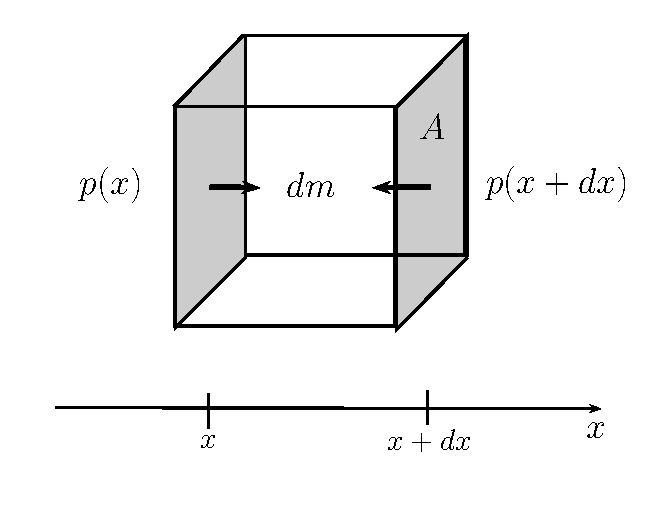
\includegraphics[width=0.3\textwidth]{newton.pdf}
  \end{center}
   \vspace{-20pt}
  \caption{}\label{fig: newton}
  \vspace{-20pt}
\end{wrapfigure}

Consider an element of (nonviscous) fluid with mass $dm$ in a volume $A dx$ (see figure \ref{fig: newton}). The force acting in the $x$-direction on surface A at $x$ due to the pressure of the surrounding fluid  is $F(x) = A p(x) $, while the force at $x +dx$ is 
\[
F(x+dx) = - A p(x+dx) = -A [p(x) + \frac{\partial p}{\partial x} dx].
\]
Here the sign is negative since the surrounding fluid pushes the element to the $-x$-direction.
The total $x$-component of the force on mass $dm$ is:
\[
dF_x = F(x) + F(x+dx) = A \left[p(x) - p(x) - \frac{\partial p}{\partial x} dx\right] = - A \frac{\partial p}{\partial x} dx.
\]  
According to Newton's law, this force creates an acceleration of the mass element $dm$:
\[
dF_x = - A \frac{\partial p}{\partial x} dx = \frac{\partial v_x}{\partial t} dm = \rho_0 A \frac{\partial v_x}{\partial t} dx
\]
with $\rho_0$ the static value of the density $\rho$. Simplifying the previous equation, and repeating the process for the $y$- and $z$-directions yields
\begin{equation}
\vec{\nabla} p = - \rho_0 \frac{\partial \vec{v}}{\partial t}.
\label{newt}
\end{equation}


\subsubsection*{Equation of continuity}
%\vspace{-15pt}
Given that mass is conserved in fluid dynamics, we can write an equation of continuity. Consider a volume element $V$ containing fluid. Any change of mass in $V$ is the result of a flow of particles in or out of this volume element. A change of mass can be written as:
\[
\frac{\partial m}{\partial t} = \frac{\partial }{\partial t} \int_{V} \rho \,dV =\int_{V} \frac{\partial \rho}{\partial t} dV
\]
Whereas the flux of particles in or out of the volume is characterised as:
\[
\Phi_m
= - \rho_0 \oint_A \vec{v} \cdot d\vec{A}
= - \rho_0 \int_{V} (\vec{\nabla} \cdot \vec{v}) \, dV.
\]
where in the last equality the divergence theorem was used.
Since the change of mass is equal to the mass flux, following relation between the density and the velocity of the particles can be obtained:
\begin{equation}
\frac{\partial \rho}{\partial t}  = - \rho_0 (\vec{\nabla} \cdot \vec{v})
\label{cont}
\end{equation}


\subsubsection*{Adiabatic gas law}
%\vspace{-15pt}
It is assumed that the motion of the fluid is an adiabatic process. In combination with the first law of thermodynamics this gives
\[
\delta Q = n C_V dT + p dV = 0.
\]
If we suppose the fluid to be an ideal gas, following equation holds:
\[
p dV + V dp = n R dT.
\]
Combining the previous equations gives
\[
(R+ C_V ) p dV + C_V V dp = 0  \qquad \textrm{ or } \qquad \gamma \frac{dV}{V} + \frac{dp}{p} = 0 \qquad \textrm{ with } \qquad \gamma \equiv \frac{R+C_V}{C_V} = \frac{C_p}{C_V}.
\]
Or in terms of the density:
\[
\gamma \frac{d(m/\rho)}{m/ \rho} + \frac{dp}{p} = -\gamma \frac{m}{\rho^2} \frac{d\rho}{m/ \rho} + \frac{dp}{p} =- \gamma \frac{d\rho}{\rho} + \frac{dp}{p} =0
\]
In the assumption that the pressure and density variations are small, the equation becomes:
\begin{equation}
\frac{dp}{p_0} =\gamma \frac{d\rho}{\rho_0}
\label{adia}
\end{equation}
with $\rho_0$ the static density and $p_0$ the mean pressure of the surroundings.





\subsubsection*{Combination of previous equations}
%\vspace{-15pt}
Combining equations (\ref{cont}) and (\ref{adia}) gives:
\begin{equation}
\frac{\partial p}{\partial t} = - p_0 \gamma \left(\nabla \cdot \vec{v}\right).
\label{dpdt}
\end{equation}
Taking the time derivative of the previous equation and substituting equation (\ref{newt}) gives
\[
\frac{\partial^2 p}{\partial t^2} =  c^2 \Delta p
\]
with $c\equiv \sqrt{\frac{p_0 \gamma}{\rho_0}}$ the speed of sound in the fluid.







%2.2 Reflection and Absorbtion
%Definition of Reflection coeff and absorbtioncoeff
%Boundary conditions (p_in + p_refl = p_trans and v_n,in + v_n,refl = v_n,trans)
\subsection{Reflection and absorption}
In acoustics, several important parameters can be determined in order to characterise the acoustical properties of an object. The  definitions of these parameters will be stated in the following paragraphs.


\subsubsection*{Characteristic impedance}
%\vspace{-15pt}
An important quantity is the characteristic impedance $Z$ of a material. It is defined as 
\[
Z = \rho c
\]
with $\rho$ the density of the medium and $c$ the longitudinal wave speed. In case of plane waves travelling through a homogeneous fluid (like air), the characteristic impedance equals the ratio of the complex pressure amplitude and the particle velocity:
\[
Z = \frac{p}{v} = \rho c
\]
where the particle velocity is evaluated in the direction of propagation.


\subsubsection*{The reflection coefficient}
%\vspace{-15pt}
When a sound wave travels from one medium to another, it will be reflected and refracted at the boundary surface. Let us consider plane longitudinal waves:
\begin{align*}
&\pin = \pinnul e^{i (\vec{r} \cdot \kin -  \omega t)}\\
&\pref = \prefnul e^{i (\vec{r} \cdot \kref -  \omega t)}\\
&\ptr = \ptrnul e^{i (\vec{r} \cdot \ktr -  \omega t)}\\
\end{align*}

Let $\thetain$, $\thetaref$ and $\thetatr$ be the angles respective to the normal of the surface of the incoming wave (in), reflected  wave (ref) and transmitted  wave (tr) respectively. The norm of the wave vectors are 
\[
\left\|\kin\right\|
= \left\|\kref\right\|
= \frac{\omega}{c_1}
\qquad\textrm{ and } \qquad
\left\|\ktr\right\|
= \frac{\omega}{c_2}
\]
with $c_1$ and $c_2$ the speeds of sound in medium 1 and 2. The acoustical waves are subject to boundary conditions at the surface. First of all, the law of action and reaction dictates that the pressure should vary continuously at the boundary: $\pin + \pref = \ptr$.
Secondly, the normal velocity of the particles remains the same in both media at the boundary, whereas the tangential component may differ: $\vin^\perp + \vref^\perp = \vtr^\perp$.

These boundary conditions result in Snell's law
\[
\left\|\kin\right\| \sin\thetain = \left\|\kref\right\| \sin\thetaref = \left\|\ktr\right\| \sin\thetatr
\]
and the following solutions in terms of the pressure reflection coefficient $R_p = p_{ref,0}/p_{in,0}$ and the pressure transmission coefficient $T_p = p_{tr,0}/p_{in,0}$ 
\[
R_p = \frac{Z_2 \cos \theta_{in} - Z_1 \cos \theta_{tr}}{Z_2 \cos \theta_{in} + Z_1 \cos \theta_{tr}} \qquad \textrm{ and } \qquad
T_p = \frac{2 Z_2 \cos \theta_{in} }{Z_2 \cos \theta_{in} + Z_1 \cos \theta_{tr}}.
\]
with $Z_1 = \rho_1 c_1$ the characteristic impedance of fluid 1 and $Z_2 = \rho_2 c_2$ the impedance of medium 2.  
The reflection coefficient ranges from $-1$ to 1, while the transmission coefficient has a value between 0 and 2. A value greater than 1 for the transmission coefficient may seem in disagreement with conservation of energy, but that is not the case. We speak of pressure coefficients, instead of intensity coefficients. 

The average acoustic intensity $\vec{I}$ of a sound wave is defined as 
\[
\vec{I} = \frac{1}{T} \int^{T}_{0}{p(t) \vec{v}(t) \,dt}.
\]
with $p$ the instantaneous pressure and $\vec{v}$ the particle velocity. It equals the sound power per unit area. For plane waves, the magnitude of the intensity becomes 
\[
I = \frac{1}{T} \int^{T}_{0}{\frac{\left(p(t)\right)^2}{Z} \,dt} = \frac{p^2_{rms}}{Z}.
\]
The reflection and transmission coefficients are then defined as
\[
R_I = \frac{I_{ref}}{I_{in}} = \frac{p^2_{ref,rms}}{Z_1} \frac{Z_1}{p^2_{in,rms}} = R_p^2 \qquad\textrm{ and } \qquad T_I = \frac{I_{tr}}{I_{in}} = \frac{p^2_{tr,rms}}{Z_2} \frac{Z_1}{p^2_{in,rms}} = T_p^2 \frac{Z_1}{Z_2}. 
\]
When $Z_1 \ll Z_2$, $T_p \approx 2$, but $T_I$ becomes 0. Hence there is no discrepancy.




\subsubsection*{The absorption coefficient}
%\vspace{-15pt}
The sound absorption coefficient is defined as the fraction of acoustic energy that is absorbed by the surface on reflection \cite[p.12]{Geetere}.  When dealing with incident plane waves, the absorption coefficient can be written as a function of the (pressure) reflection coefficient:
\begin{equation}
\alpha(\theta_{in}) = 1 - \left|R_p(\theta_{in})\right|^2.
\label{absorption}
\end{equation}











\begin{comment}
\end{document}
\end{comment}

\section{Scale model of a noise barrier}
A scale model of a simple noise barrier is investigated to characterize several aspects such as the reflection and diffraction of incident sound.

\subsubsection*{The noise barrier}
The model under consideration is composed of five wooden blocks of dimensions $212\,\mathrm{mm} \times 212\,\mathrm{mm} \times 60\,\mathrm{mm}$. These are positioned side by side to form a barrier that is $1.06\,\mathrm{m}$ long.

This could realistically be a 1:10 scale model of a noise barrier that is 2.12\,m high and 60\,cm wide. 

\subsubsection*{The excitation source}
Working with a 1:10 scale model also means that the wavelengths to be considered should be reduced by a factor of 10.

A suitable means of excitation was found in a small spark source. This produces a signal with sufficiently high frequencies and it is an excellent approximation for an ideal point source.

\figOctaveTwo[htb]{sparkSourcePlots}{Characteristics of the spark source}
	{sparkImpulseResponse}{impulse response}
	{sparkSpectrum}{spectrum}



[foto's, schets]

\subsubsection*{Capturing the sound field}
A programmable $x$-$y$-positioning system was used in order to scan a grid of measurement points in front of and behind the wall. The sound field at each measurement point was recorded with a high frequency microphone connected to an oscilloscope sampling at 5\.MHz. The triggering was based on the sudden spike caused by the electromagnetic pick up of the spark on the microphone wires, this accurately defined the moment when the spark was emitted.

Because of the very low acoustic energy associated with a single spark, additional pre-amplification was required. Even then, the signal to noise ratio was extremely low. In fact, for the lowest measurement point right behind the wall, the signal to noise ratio was of the order of one in ten!

In order to get a sufficiently clean signal at each point of the grid, each measurement was averaged over a thousand excitations. Even then, significant noise remained, especially in the measurements right behind the wall.

Figure \ref{rawSparkMeasurements} shows two averaged signals as they were received by the microphone during a measurement right behind the wall, at a distance of 10\,cm behind the wall, at both the lowest (and hence the most attenuated) and the highest (least attenuated) measurement point.

Note that the $s/n$ ratio in the time domain plot (fig \ref{measurementsRightBehindWall}) of the red graph is abysmal. This noise, however, seems to have a fixed pattern. A glance at the spectrum in figure \ref{spectraMeasurementsRightBehindWall} shows that this noise occurs at specific frequencies that are harmonics of 52\,kHz. Due to the very high amplification of the weak signal and the low $s/n$ ratio of a single measurement, any present noise that was in sync with the triggering became very significant in the averaged signal. The origin of this noise is possibly to be found in electromagnetic pick up from the spark generator, which charges a capacitor by pulsing it with high voltage spikes at a fixed frequency.


\figOctaveTwo[htb]{rawSparkMeasurements}{Resulting signal of an averaged 1000 measurements of the scale model. The measurement was obtained closest behind the wall (10\,cm distance) at the lowest (red, 3\,cm high) and highest point (blue, 24\,cm high, 3\,cm above the wall). Notice the persistent parasitic noise at the harmonics of 52\,kHz.}
	{measurementsRightBehindWall}{time domain}
	{spectraMeasurementsRightBehindWall}{frequency domain}

Averaging even more than a thousand measurements could potentially improve the $s/n$ ratio further. However, the resulting measurement times would quickly become intractable and the noise spikes at the harmonics of 50kHz would remain nonetheless.

Apart from this high frequency noise, there were also low frequency components present. The high magnification made the pick up noise at 50\,Hz (and harmonics thereof) prominent, as can be seen in figure \ref{measurementsLowFreqNoise}. Occasionally also was an additional low frequency attribution, often manifesting itself right after the trigger peak. This is possibly the response of the measurement chain on the high impulse spike created by the electromagnetic pick up of the spark by the microphone wires. This sudden spike was, in fact, order of magnitude larger than the actual signal.

All the factors above mean that with our setup, we could only get reliable spectral data in the 5\,kHz to 40\,kHz area, corresponding to 500\,Hz to 4\,kHz life sized. In order to go beyond this frequency band, a stronger and better shielded spark source is advised.

The results from the scale model will be discussed in depth in section \ref{sectComparison}, in tandem with the results from the simulation discussed below.


XXX Deconvolving to get rid of floor (so pure point source/plane wave approaching) was unsuccessful


TODO attenuationcorrection


% vim: spell spelllang=en_us

\section{Numerical simulation}
With the ever increasing strength of modern computers, it has become feasible to make accurate simulations of physical systems. This is often more practical than building an actual physical (scale)model.


\subsection{Finite difference time domain method}
In this section, we describe an implementation of a finite difference time domain (FDTD) method. This is a simple and intuitive way of simulating the progression of acoustic waves through a medium (in our case, air) that allows one to easily implement obstacles (eg. a hard floor, a wall). For simplicity, an infinitely long barrier on an infinitely large floor is assumed. The problem thus reduces to two dimensions.

The FDTD method consists of simulating the pressure field, $p$, and velocity field, $\vec{v} = (v, w)$,  on a discrete spacial grid. The basic equations that govern the evolution of these fields are equations \ref{newt} and \ref{dpdt}, which in two dimensions read
$$
\pderiv{v(x,y,t)}{t} = -\frac{1}{\rho} \pderiv{p(x,y,t)}{x}
, \qquad
\pderiv{w(x,y,t)}{t} = -\frac{1}{\rho} \pderiv{p(x,y,t)}{y}
$$
$$
\pderiv{p(x,y,t)}{t} = -\rho c^2 \left(\pderiv{v(x,y,t)}{x} + \pderiv{w(x,y,t)}{y}\right)
$$
where we used $c^2 = p_0 \gamma / \rho$. These equations will be discretized in space and time. We use the shorthand notation $\pnij$ to denote $p(x_i, y_j, t_n)$. The velocities $\vnij$ and $\wnij$ are defined analogously. The above equations can now be discretized as a central difference
$$
\frac{\vij^{n+1} - \vij^{n-1}}{2\Dt} = -\frac{1}{\rho} \frac{\pn_{i+1,j} - \pn_{i-1,j}}{2\Dx}
, \qquad
\frac{\wij^{n+1} - \wij^{n-1}}{2\Dt} = -\frac{1}{\rho} \frac{\pn_{i,j+1} - \pn_{i,j-1}}{2\Dy}
$$
$$
\frac{\pij^{n+1} - \pij^{n-1}}{2\Dt} = 
	-\rho c^2 \left(
		\frac{\vn_{i+1,j} - \vn_{i-1,j}}{2\Dx}
		+ \frac{\wn_{i,j+1} - \wn_{i,j-1}}{2\Dy}
	\right)
$$
Here, $\Dt$ is the temporal discretization, and $\Dx$ and $\Dy$ are the spatial discretizations.

An improvement on the accuracy can be made by shifting the pressure and velocity grids by half a step in the appropriate dimensions (spacial and temporal). This is called a \emph{staggered grid}\cite{staggered-grid}, and is described by the transformation
$$
\vnij \to v_{i,j+\half}^{n+\half}
, \qquad
\wnij \to w_{i+\half,j}^{n+\half}
, \qquad
\pnij \to \pn_{i+\half, j+\half}
$$
This allows one to take the central derivatives over half the interval of before, as if the discretization length has halved
$$
\frac{v_{i,j+\half}^{n+\half} - v_{i,j+\half}^{n-\half}}{\Dt}
	= -\frac{1}{\rho} \frac{\pn_{i+\half,j+\half} - \pn_{i-\half,j+\half}}{\Dx}
$$
$$
\frac{w_{i+\half,j}^{n+\half} - w_{i+\half,j}^{n-\half}}{\Dt}
	= -\frac{1}{\rho} \frac{\pn_{i+\half,j+\half} - \pn_{i+\half,j-\half}}{\Dy}
$$
$$
\frac{p_{i+\half,j+\half}^{n+1} - p_{i+\half,j+\half}^{n}}{\Dt} = 
	-\rho c^2 \left(
		\frac{v_{i+1,j+\half}^{n+\half} 
			- w_{i,j+\half}^{n+\half}}{\Dx}
		- \frac{w_{i+\half,j+1}^{n+\half} 
			- w_{i+\half,j}^{n+\half}}{\Dy}
	\right)
$$
These equations can now easily be solved for $p^{n+1}_{i+\half, j+\half}$, $v_{i,j+\half}^{n+\half}$ and $w_{i+\half,j}^{n+\half}$ to derive the update rules for the simulation.

Lastly, for this method to be stable, a constraint is imposed on the temporal and spacial discretization. Stability ensues only if the Courant-Friedrichs-Lewy condition is satisfied\cite{courant-friedrichs-lewy}\cite{numerical-stability-2D-FDTD}
$$
c\Dt \leq \left[\frac{1}{(\Dx)^2} + \frac{1}{(\Dy)^2}\right] ^ {-1/2}
$$
In our case, we fixed $\Dx = \Dy = h$ and chose $\Dt$ as the largest number to satisfy the above relation:
$$
\Dt = \frac{h}{\sqrt{2}}
$$


\subsection{Modelling the physical scale model}
The scale model setup discussed earlier will be represented in the general framework from the previous section.

\subsubsection*{The grid}
The setup of the grid is summarized in table \ref{gridSetup}.


\begin{table}[htb]
\begin{center}
\caption{The setup of the grid for the finite difference time domain simulation of the scale model\label{gridSetup}}
\begin{tabular}{c|c|c}
Measurement&	In front of wall&	Behind wall\\\hline
grid dimensions&
	$3.3\,\mathrm{m} \times 1.4\,\mathrm{m}$&
	$2.8\,\mathrm{m} \times 1.3\,\mathrm{m}$\\
spacial discretization $h$&
	$0.3\,\mathrm{mm}$&
	$0.25\,\mathrm{mm}$\\
temporal discretization $\Dt$&
	$0.62\,\mu\mathrm{s}$&
	$0.52\,\mu\mathrm{s}$\\
grid size in points&
	$11000 \times 4667$&
	$11200 \times 5200$\\
position of source from left boundary&
	$0.75\,\mathrm{m}$&
	$0.60\,\mathrm{m}$\\
distance from source to wall&
	$2.0\,\mathrm{m}$&
	$1.2\,\mathrm{m}$\\
\end{tabular}
\end{center}
\end{table}

The height of the excitation source was 15\,cm in both setups, which is the height of the actual spark source used in the scale model measurements.

A visual representation of the geometry of the grids is given in figure \ref{simulationGrids}.

\figOctaveTwoVariableSpace{-0.9cm}{simulationGrids}{Visualisation of the grids used in the simulations. The mesh of points correspond to the measurement positions. The source position is indicated as a single point.}
	{gridBeforeWall}{measurements in front of the wall}
	{gridBehindWall}{measurements behind the wall}




\subsubsection*{The excitation}
The excitation signal consisted of a temporal impulse shaped like a hanning function with a duration of 25\,$\mu$s. This is sufficiently long to avoid temporal discretization artifacts, and sufficiently short to cover all the frequencies we are interested in. This time also approximates the duration of the actual spark used in the scale model measurements.

To avoid spatial discretization artifacts, the excitation was spread out over a two dimensional gaussian with a width $2\sigma$ of 3\,mm. This proved to be a good trade-off between a perfect point source and excessive discretization artifacts. Note that the spark gap of the spark source used in the experiment had a comparable size of 3\,mm.

\figOctaveTwo[htb]{simuExcitationPlots}{Characteristics of the excitation signal of the simulation}
	{simuImpulseResponse}{impulse response}
	{simuSpectrum}{spectrum}

The excitation signal was applied as a soft 
source\cite{soft-hard-source} by simply adding it to the 
pressure field. Because the excitation is merely added to the pressure 
field, and not forced (as for hard sources), the actual signal that will be 
radiated from the source point will not be equal to the excitation signal 
itself. It will be altered by the response of the system. A virtual free 
field measurement was performed to characterize the total resulting 
excitation signal. The results are shown in figure \ref{simuExcitationPlots}.They can be compared to the actual spark source used in figure \ref{sparkSourcePlots}. 


[TODO plots: imagesc van gaussische?]


\subsubsection*{The boundaries}
The entire space was modelled to have perfectly reflecting edges as boundaries. The wall acting as the noise barrier was also modelled to be perfectly reflecting (ie. having an infinite impedance). This was accomplished by forcing the velocity parallel to the surface to be zero. For example, for the floor this means $w_{i,0}^n = 0$ and for the left wall this means $v_{0,j}^n = 0$ (for all $n$, $i$ and $j$).



\subsection{Matching 2D simulation with 3D scale model}
Given the large amount of symmetry, the situation lent itself perfectly for simulation in two dimensions. However, this also means that there are some discrepancies when compared to the 3D scale model.

The most profound difference is the fact that the pressure signal of a point source in 2D (or a line source in 3D) has a $1/\sqrt{r}$ geometrical attenuation, whereas a point source in 3D has a $1/r$ dependency, with $r$ the distance traveled. In order to be able to compare the simulation with the scale model, an extra correction of the pressure amplitudes was made to factor in the energy radiated away in the third dimension in a 3D setup.
$$
\pij^{\mathrm{3D}}(t) = \frac{\pij(t)}{\sqrt{ct}}
$$
Note that this correction was applied afterwards on the data of the finished the simulation, not while it was running. In every result that follows, we used the corrected pressure amplitudes $\pij^{\mathrm{3D}}$. [TODO even when we mention $\pij$?]

Additional discrepancies may occur if, for example, there are diffuse reflections on the wall in the 3D case. Those may still reach the observer and contribute to the signal, but they are not accounted for in the 2D case. However, in our case of a hard and flat wall, such effects are not expected to play a significant role.

% vim: spell spelllang=en_us

\section{Comparison of scale model with simulation \label{sectComparison}}

\subsection{Detailed results for several measurement positions}
The results of several measurements in front of the wall are shown in figure \ref{beforePlots}. Measurements at a similar position, but with the setup for the measurements behind the wall are shown in figure \ref{behindPlots}.


\begin{figure}
\figOctaveTwoNoFigNoCaption{-0.0cm}
	{before-x8-y1}{$x$ = 28\,cm, $y$ = 6\,cm}
	{before-x8-y3}{$x$ = 28\,cm, $y$ = 12\,cm}
\figOctaveTwoNoFigNoCaption{-0.0cm}
	{before-x8-y5}{$x$ = 28\,cm, $y$ = 18\,cm}
	{before-x8-y7}{$x$ = 28\,cm, $y$ = 24\,cm}
\caption{Results of a selection of measurements 28\,cm in front of the wall, at different heights. The curves plotted are the raw measurement without (red) and with (green) correction for the attenuation of high frequencies, and the result of the simulation (black). \label{beforePlots}}
\end{figure}

\begin{figure}
\figOctaveTwoNoFigNoCaption{-0.0cm}
	{behind-x6-y1}{$x$ = 28\,cm, $y$ = 6\,cm}
	{behind-x6-y3}{$x$ = 28\,cm, $y$ = 12\,cm}
\figOctaveTwoNoFigNoCaption{-0.0cm}
	{behind-x6-y5}{$x$ = 28\,cm, $y$ = 18\,cm}
	{behind-x6-y7}{$x$ = 28\,cm, $y$ = 24\,cm}
\caption{Results of a selection of measurements 28\,cm behind the wall, at different heights. The curves plotted are the raw measurement without (red) and with (green) correction for the attenuation of high frequencies, and the result of the simulation (black). \label{behindPlots}}
\end{figure}


\subsubsection*{Measurements in front of the barrier}

The spectra in figure \ref{beforePlots} show a very harsh comb filter shape due to the rather long delay between the direct sound and the reflected sound. This kind of filter is generally considered to give a harsh sound, and hence it makes sense for a noise barrier to not only prevent transmission (and diffraction), but also to prevent reflection back to the sound source.

Apart from the obvious fast comb effect, there is also `slow' comb visible in the plots, due to the short time delay between the directly incident sound and the sound that reflected via the floor first.

The time domain plots give an indication of the reflected signal. The reflected peak at 6.7\,ms is clearly smaller in figure \ref{behind-x6-y7} than it is in the other figures. The peak in this case is completely ascribed to diffraction at the edge of the wall (or diffuse relfections), as there is no direct path available through (specular) reflections.

Notice that the spectra and time domain signals follow the general pattern of the simulated data, though the (air attenuation corrected) spectra are consistently higher than the simulated values. This is a possible result of deviting values of the temperature and humidity during the measurements, as these took about 12 hours and were done overnight. Hence the correction may have been too strong. The uncorrected spectra did not exceed those of the simulation.



\subsubsection*{Measurements behind the barrier}

Figure \ref{behindPlots} shows some results of the measurement setup where the measurements were made behind the wall. Here the corrected spectra match the simulated spectra more intimately.

Figure \ref{behind-x6-y1} represents a low measurment, where we see two sets of peaks one at 4.3 and 4.5\,ms and a second set at 4.6 and 4.8/,ms. Each set is the result of the diffraction over the top of the wall of (1) the direct sound of the source to the top of the wall, and (2) the diffraction of the sound that reached the top of the wall by first reflecting at the floor. The second set of peaks are a diffracted signal that first reflected of off the floor before reaching the microphone. Measurements that were made on higher positions from the floor have these two sets of peaks further apart.

TODO : refer to figure

The high frequency regime of the spectrum in figure \ref{behind-x6-y1} shows an attenuation of 20\,dB per decade. This is consistent with the rule of thumb of equation \ref{diffractionEq}, which predicts a characteristic frequency $f_0$ of 1.8\,kHz.

This attenuation due to diffraction can also be found in figures \ref{behind-x6-y3} and \ref{behind-x6-y5}, though in a lesser degree. In figure \ref{behind-x6-y7}, there is a direct path from source to microphone, and this vastly overpowers the small diffraction peaks that are still present (where the diffracted signal reflected of off the floor on the side of the microphone).

Note that the second set of peaks in figure \ref{before-x8-y7} also have this characteristic attenuation due to the diffraction.




\subsection{Global overview of the sound field around the wall}
Figures \ref{band1}, \ref{band2}, \ref{band3} and \ref{band4} give a visual representation of the characteristics of the wall on various spatial coordinates. Each figure represents the intensities in a fixed octave band. All intensities are normalized to the maximum of all considered octave bands so they can be compared.

The white areas in the experimental graphs represent lacking data (due to a technical error during the measurement). Also note that the frequency range in figure \ref{bands1} is bordering on the frequency range where measurement noise becomes significant, hence the rather large deviation from the simulated graph in figure \ref{bandsSim1}

In figure \ref{band2}, the frequencies under consideration are comparable to the width of the wall. Compared to the high frequency regime of figure \ref{band4}, noticably more intensity can be found behind the barrier due to diffraction. However, these lowest spectral bands (figure \ref{band1} and \ref{band2}) are only on the onset of diffraction. It would have been interesting to examine even lower frequencies, where the wavelength becomes comparable to the \emph{height} of the barrier. Sadly, the data in that frequency regime was not usable due to excessive noise. The comb-like shape of the spectrum also prevents from assigning a representative value to the average intensity in the small (absolute, linear) frequency span of those lower octave bands. This, by itself, also explains the noisy appearance of figure \ref{bands1}.




This slow

SOLVE?
DECONVOLVING DID NOT WORK






\begin{figure}
\figOctaveTwoVariableSpaceNonFig{-1.0cm}{band1}{Intensity (dB) in the 2.5\,kHz to 5\,kHz octave band.}
	{bands1}{measured}
	{bandsSim1}{simulated}
\figOctaveTwoVariableSpaceNonFig{-1.0cm}{band2}{Intensity (dB) in the 5\,kHz to 10\,kHz octave band.}
	{bands2}{measured}
	{bandsSim2}{simulated}
\figOctaveTwoVariableSpaceNonFig{-1.0cm}{band3}{Intensity (dB) in the 10\,kHz to 20\,kHz octave band.}
	{bands3}{measured}
	{bandsSim3}{simulated}
\figOctaveTwoVariableSpaceNonFig{-1.0cm}{band4}{Intensity (dB) in the 20\,kHz to 40\,kHz octave band.}
	{bands4}{measured}
	{bandsSim4}{simulated}
\end{figure}






\begin{comment}
\documentclass[12pt,a4paper]{article}
\usepackage{a4wide}
\usepackage{amsfonts, amsmath, amsthm}
\usepackage[english]{babel}
\usepackage{framed}
\usepackage[pdftex]{graphicx}
\usepackage{epstopdf}
\usepackage[font=small,format=plain,labelfont=bf,up,textfont=it,up]{caption}
\usepackage{wrapfig}
\usepackage{tocloft}
\usepackage{psfrag}
\usepackage{subfig}
\usepackage[latin1]{inputenc}
\usepackage{verbatim}

%\usepackage{bbold}
\usepackage{bbm}
\topmargin -15mm
\textwidth 16truecm
\textheight 24truecm
\setlength\parindent{0pt}
\setlength\parskip{0.20in plus0.05in minus0.05in}
\newcommand{\Z}{\mathbb{Z}}
\newcommand{\N}{\mathbb{N}}
\newcommand{\R}{\mathbb{R}}
\newcommand{\C}{\mathbb{C}}
\newcommand{\eps}{\varepsilon}
\fboxrule 1pt
\fboxsep 7pt
\pagenumbering{arabic}
%3. In situ measuments of the reflection coefficient

%3.1 Adrienne method
%General intro, definition of reflection coeff
%Problems: directivity, no speakerdeconvolution

%3.2 Our method
%3 meters between mic and speaker
%3,15 meters high, not practical
%Helmholtz resonator

%3.3 Mls vs sweep
%mls16x64 - mls18x16 - sweep1X64 - sweep60

%3.4 Diffraction
%Measurement on the side of the wall?

%3.5 Our results vs Adrienne?

\begin{document}
\end{comment}


\section{In situ measurements of the reflection coefficient}
One of the objectives of our project was to develop a program in Matlab to record and process several acoustic signals to determine the sound characteristics of a wall. 
This section contains a description of our method; an assessment of the standard measuring method (the Adrienne method) and the results of an in situ measurement. 

\subsection{Recording method}
The particulars regarding the measurement equipment will be discussed in the following section; as well as the methods of data gathering and processing. Furthermore, a short description of possible excitation signals will be given and finally the developed method will be put to the test by measuring the absorption characteristics of a Helmholtz resonator.

\subsubsection{Recording equipment}
% Weet niet goed wat er hier allemaal moet staan
The following hardware was used during the experiments:
%\vspace{-20pt}
\begin{itemize}
	\setlength{\itemsep}{1pt}
  \setlength{\parskip}{0pt}
  \setlength{\parsep}{0pt}
	\item Octa-Capture sound card by Roland.
	\item Amplifier.
	\item Zircon loudspeaker.
	\item 1/2" Condenser Microphone Cartridge Type 4130 with Microphone Preamplifier Type 2642.
\end{itemize}

\begin{wrapfigure}{r}{0.2\textwidth}
	%\vspace{-20pt}
  \centering
    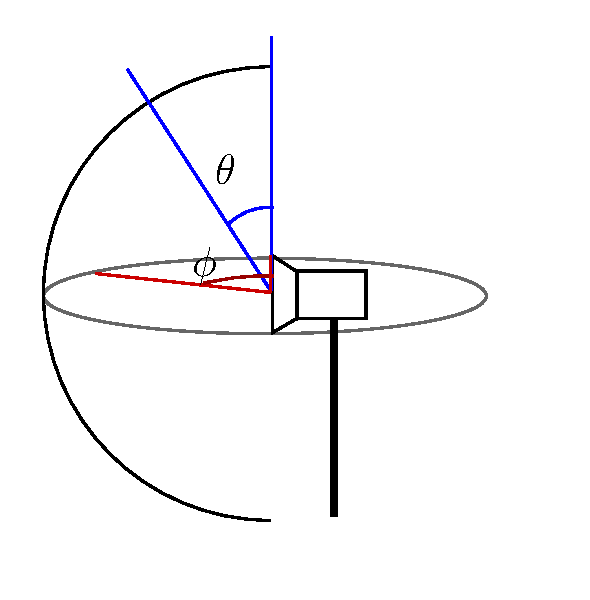
\includegraphics[width=0.2\textwidth]{thetaphi.pdf}
  \caption{Definition of angles $\theta$ and $\phi$.}
  \label{fig: thetaphi}
  %\vspace{-40pt}
\end{wrapfigure}
The software necessary to play and record sounds with these instruments was written in Matlab using the Data Acquisition Toolbox. The subsequent processing of these signals was also done in Matlab. The general content of this software will be discussed in section \ref{processing}. But in order to do accurate measurements, the specifics of the speaker have to be examined.

The impulse and frequency response of the Zircon speaker are shown in figure \ref{fig: ZirconImp}. The impulse response is rather short (less than 4 ms) and the frequency response has a smooth magnitude. To determine these responses, the measurement was performed in front of the speaker. However, the speaker is not omnidirectional; figures \ref{fig: thetavar} and \ref{fig: phivar} show the frequency response at different vertical and horizontal angles. The definition of the angles is given in figure \ref{fig: thetaphi}. 
\begin{figure}[h!]
  \centering
  \subfigure[Impulse response]{\label{fig: Zirconimp}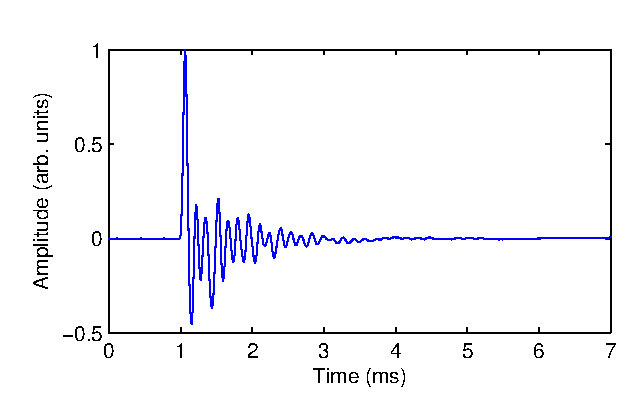
\includegraphics[width=0.45\textwidth]{ZirconImp}}                
  \subfigure[Frequency response]{\label{fig: Zirconspec}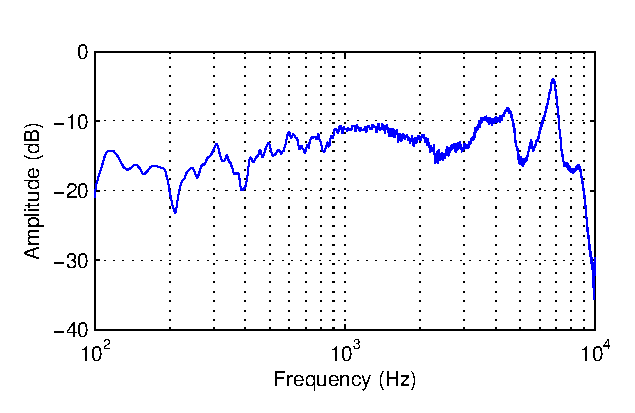
\includegraphics[width=0.45\textwidth]{ZirconSpec}}
  \caption{Impulse response and magnitude of the frequency response of the Zircon loudspeaker. The measurement was done in front of the speaker. }
  \label{fig: ZirconImp}
\end{figure}


It is clear that the speaker is very directional; when doing measurements, one should keep this in mind. For $\theta$ and $\phi$ between $75^{\circ}$ and $105^{\circ}$, the frequency response is approximately constant (per frequency). Thus when the measured sound is reflected within that solid angle, the received signal of the speaker can be considered the same for those reflecting surfaces.

\begin{figure}[h!]
  \centering
    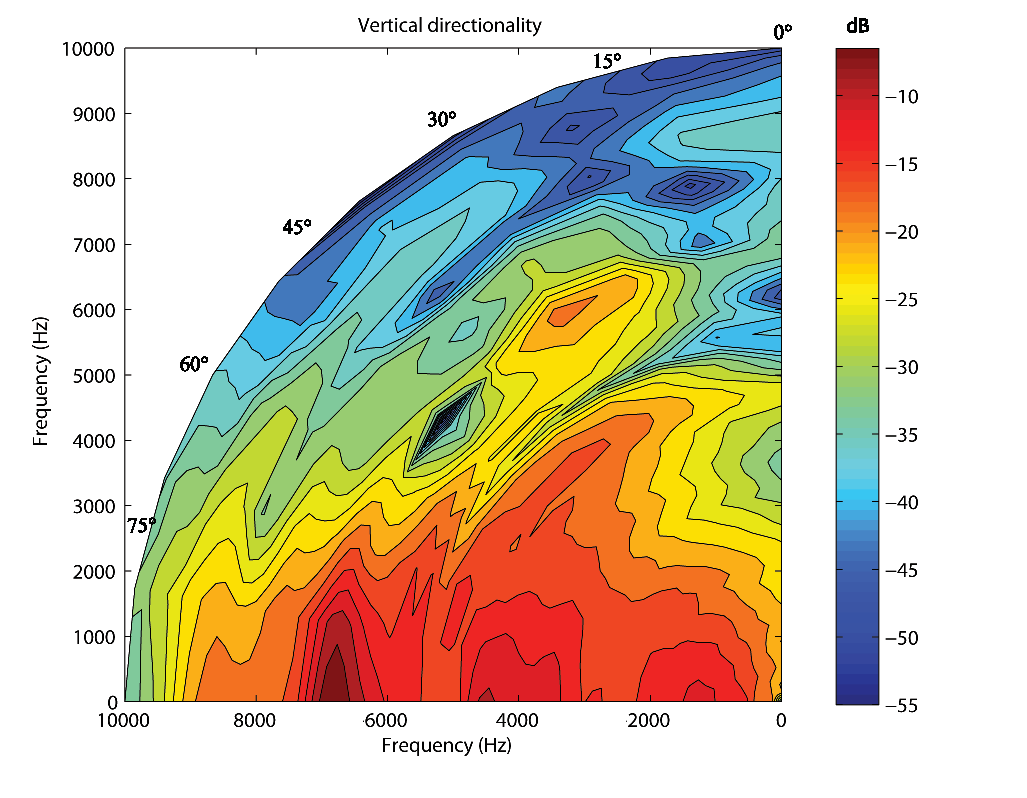
\includegraphics[width=0.8\textwidth]{thetavar1}
  %\vspace{-10pt}
  \caption{Frequency response of the Zircon loudspeaker for different vertical angles. The radial coordinate represents the frequency, the angle corresponds to the value of theta on figure \ref{fig: thetaphi}. The colour gives the magnitude of the spectrum in dB.}
  \label{fig: thetavar}
  %\vspace{-30pt}
\end{figure}

\begin{figure}[h!]
  \centering
    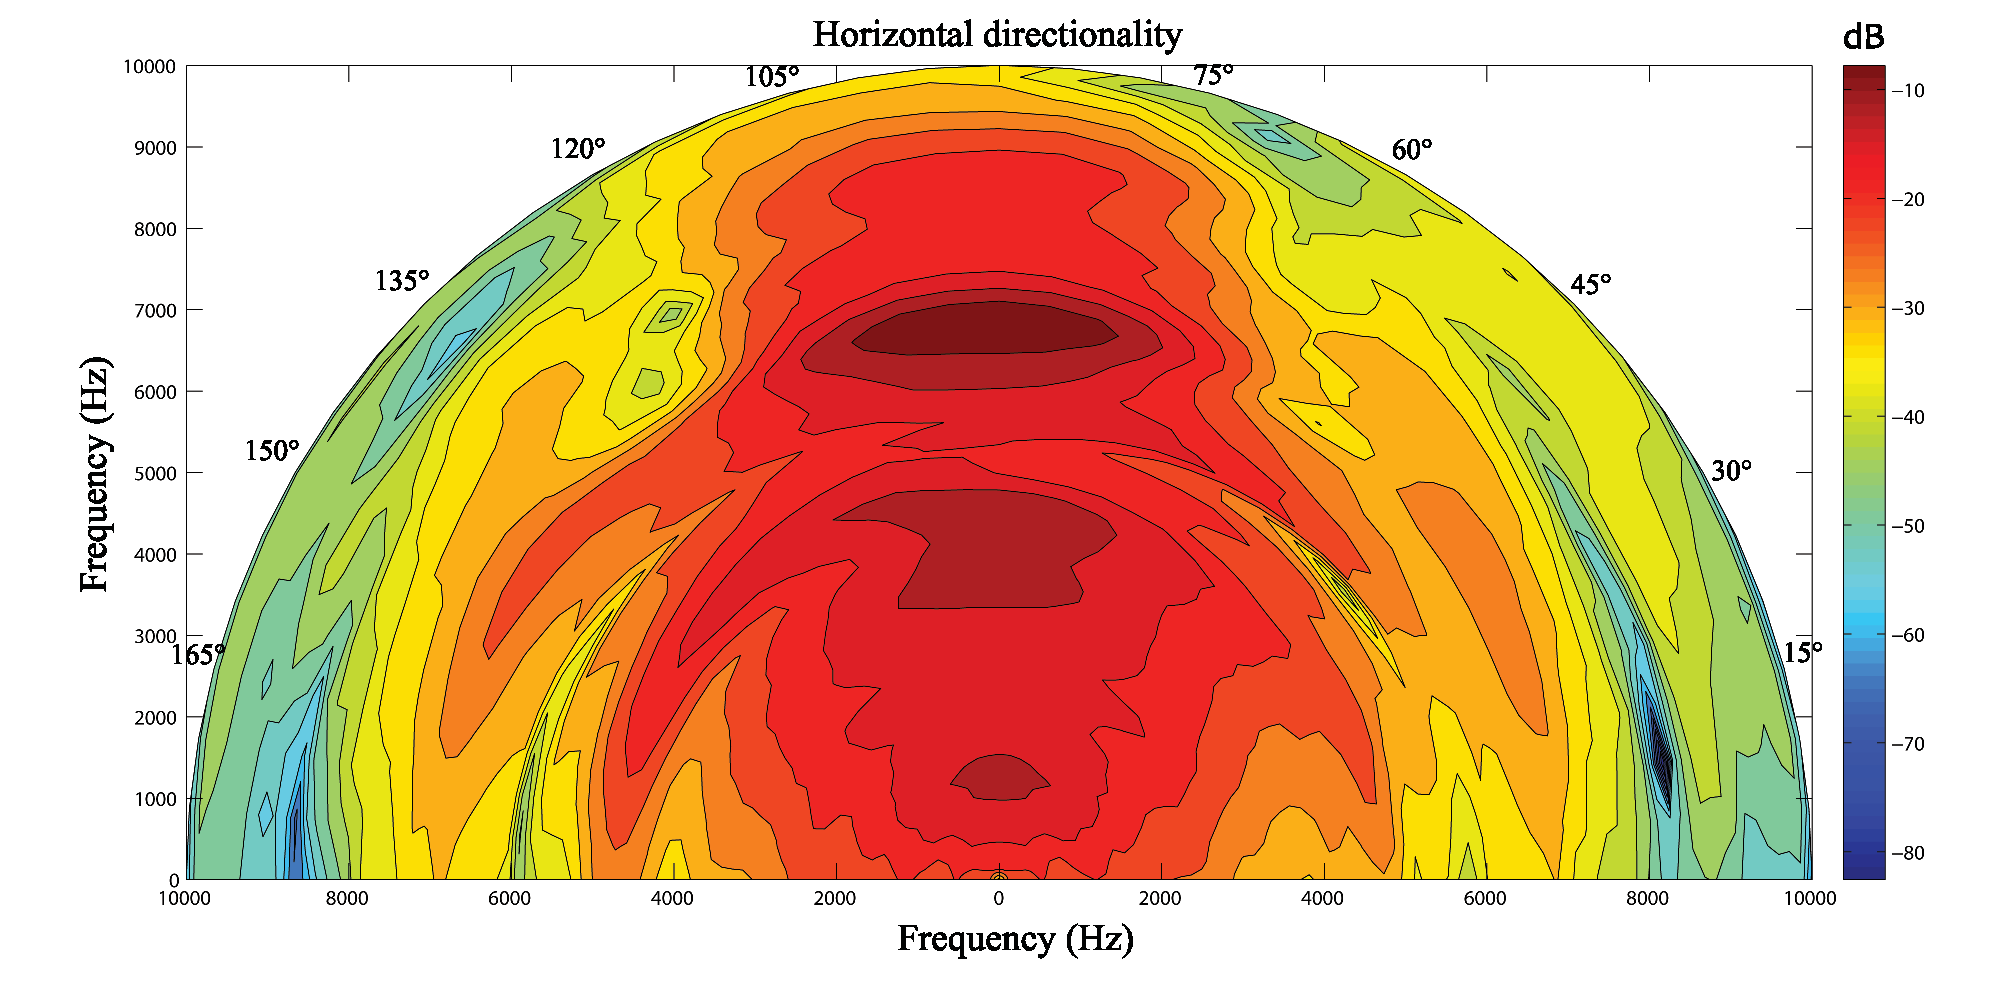
\includegraphics[width=\textwidth]{phivar1}
  %\vspace{-10pt}
  \caption{Frequency response of the Zircon loudspeaker for different horizontal angles. The radial coordinate represents the frequency, the angle corresponds to the value of phi on figure \ref{fig: thetaphi}. The colour gives the magnitude of the spectrum in dB.}
  \label{fig: phivar}
  %\vspace{-30pt}
\end{figure}




\subsubsection{Data processing}\label{processing}
The content of our Matlab program will be briefly discussed in the following paragraphs. 
\subsubsection*{Recording}
%\vspace{-15pt}
The program is capable of sending a signal to the loudspeaker while simultaneously recording the 8 analog inputs of the Octa-Capture sound card. The signals are not recorded synchronous, a (variable) delay of tens of  milliseconds is possible. Hence a reference signal should be added at the beginning of the excitation in order to render synchronization possible.

There are 2 modes of recording: the first one averages $n$ successive measurements on the spot. The excitation signal is sent to the speaker and the resulting sound is recorded. The obtained signal is then synchronized with the previous recordings by determining the peak in the cross-correlation of both signals and shifting accordingly. An additional step will be carried out to synchronize on a sub-sample time scale by means of fourier interpolation. The signal is subsequently added to the average and the cycle continues. This method gives small files, but is rather time-consuming because the signals have to be synchronized.

The second method consists of repeating the excitation signal $n$ times while recording. The averaging has to be done separately and hence the poor  measurements can be filtered out of the average. The disadvantage of this method is that the files become rather large (100\,MB for 64 sweeps of 1 second), but this is compensated by the fact that the measurement time is very short.



\subsubsection*{Impulse and frequency response}
%\vspace{-15pt}
The next step in the process is the determination of the impulse and frequency responses. The method to determine the response of the system (with speaker) is dependent on the excitation signal and will be discussed in \ref{exc}. In order to procure the response of the device under test, one has to remove the parasitic reflections. This can be done by putting a time window on the signal. The length of the window determines the lowest possible frequency for which the frequency response can be extracted from the signal. The longer the window, the better. The window which we use in our program is based on the Adrienne temporal window (see \ref{adrwindow}). The length of the window can be adjusted by changing the length of the flat portion and the trailing end, while keeping the ratio of the lengths 7/3.

To remove the direct sound from the impulse response, our program uses the subtraction method. This method requires a free field measurement of the direct sound: the direct sound is measured with the microphone and speaker in the same relative position as during the reflection measurement, but without nearby reflecting surfaces. The impulse response with reflections is first synchronized with the free field impulse response. Secondly, the free field measurement is subtracted from the signal. The resulting impulse response (which contains only the reflected component) is then windowed with an Adrienne window. Both the impulse responses are corrected for attenuation due to travel distance by multiplying the impulse response with the travel time. And finally, the frequency response of the reflecting device is determined by dividing the fourier transform of the resulting windowed impulse response by the fourier transform of the windowed free field impulse response. The last step is necessary to remove the influence of the speaker from the measured signal.



\subsubsection{Excitation signal}\label{exc}
In the domain of acoustics, the two most prominent types of excitation signals are the Maximum Length Sequence (MLS) and the frequency sweep.
This section contains a short description of both signal types and the way to calculate the impulse response from them. 


A MLS is a periodic pseudo-random binary signal with almost the same characteristics as white noise \cite{Stan}. A more theoretical description of the maximum length sequence can be found in \cite{mls}.  In order to recover the system response, the recorded signal has to be circularly cross-correlated with the input MLS. According to \cite{Stan}, any disturbing components (not correlated with the MLS) in the measured output will be phase randomized and hence appear as uniformly distributed noise along the impulse response in stead of localized peaks in the time domain. This additional noise can be reduced by averaging over multiple MLS periods. The problem with MLS is the fact that distortion artifacts (peaks) appear in the impulse response as a result of the non linearities inherent to (mainly) the loudspeaker \cite{Geetere}. These additional peaks in the impulse response can not be removed by averaging over multiple periods because it is correlated with the input signal.

The second type of excitation signal is the frequency sweep. The excitation signal consists of a sine function with a frequency growing in time. To obtain the impulse response of a system excited with a sweep, one has to deconvolve the original sweep from the measured signal. This is done by dividing the spectrum of the output by the spectrum of the sweep. This procedure can cause difficulties because of dividing by zero. The remedy for this problem is placing a window in the frequency domain. The window we use in our data processing is a hyperbolic tangent window. It is defined as:
\[
w(f) = (0.5 + 0.5 \tanh(f - f_1)/a_1)) \cdot (0.5 + 0.5 \tanh(-(f - f_2)/a_2))
\]
with $f_1$ the lower and $f_2$ the upper frequency bounds. The parameters $a_1$ and $a_2$ determine the width of the transitions and control the steepness of the window.

The advantage of the sine sweep excitation is that the distortion artifacts due to non linear behaviour appear before the linear response (as a result of linear deconvolution) and can be removed by time windowing \cite{Geetere}.  Moreover, the signal-to-noise ratio\footnote{The signal to noise ratio is defined as the ratio (in dB) between the average power of the signal recorded by the microphone and the average
power of the noise and distortions present in the tail of the deconvolved (linear) impulse response.} for the sine sweep method is larger since the impulse response has no distortion artifacts in its tail \cite{Stan}.   However, the presence of impulsive noise compromises the impulse response and these residual peaks will not be properly eliminated when using signal averaging techniques. Therefore it is concluded in \cite{Stan} that the MLS excitation signal gives more accurate results in  the presence of non white noise, whereas the sine sweep gives better results in quiet environments. 






\subsubsection{Helmholtz resonator}

\begin{wrapfigure}{r}{0.3\textwidth}
	%\vspace{-60pt}
  \centering
    \includegraphics[width=0.3\textwidth]{helmh}
  \caption{Experimental setup for the measurement of the characteristics of the Helmholtz resonator panel.}
  \label{fig: helmh}
  %\vspace{-20pt}
\end{wrapfigure}
In order to check the consistency of our program, a measurement was performed to determine the (known) absorption characteristics of a Helmholtz resonator panel. The experimental setup is presented in figure \ref{fig: helmh}. The Zircon loudspeaker is positioned at an angle of $30^{\circ}$ with  respect to the horizontal. This is to ensure that both the resonator panel and the microphone receive a similar signal from the speaker.

Figure \ref{helmsub} shows the results of a measurement with a MLS of order 16 as excitation signal which was averaged 64 times. The graph 
 contains the impulse response of the system, the free field impulse response, the subtracted signal and the used Adrienne temporal window. Figure \ref{helmspec} shows the spectrum of the subtracted signal deconvolved with the free field impulse response. The hyperbolic tangent window seen on the same figure was used to determine the impulse response of the Helmholtz resonator panel shown in figure \ref{fig: helmimp}.
 
  

\figOctaveTwo{helm}{Impulse responses of the measurements and frequency response of the Helmholtz resonator panel.}
	{helmsub}{Total (red), free field (green) and subtracted (black) impulse responses and the Adrienne temporal window (blue).}
	{helmspec}{Spectrum of the Helmholtz resonator (blue) and the hyperbolic tangent window (green).}


\begin{figure}[h!]
  \centering
    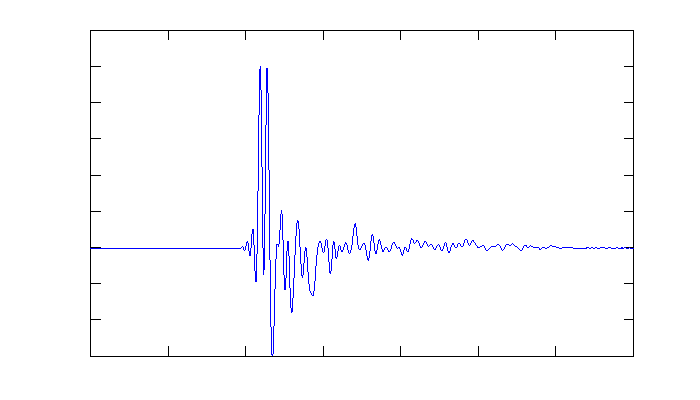
\includegraphics[width=\textwidth]{helmimp}
  %\vspace{-10pt}
  \caption{Impulse response of the Helmholtz resonator panel.}
  \label{fig: helmimp}
  %\vspace{-30pt}
\end{figure}

The frequency dependent absorption coefficient is computed using equation \ref{absorption}. The result of this calculation is displayed in figure \ref{fig: helmholtzalles} as the red line. The other lines represent measurements with other excitation signals: the yellow line is obtained as the average of 16 excitations with an MLS of order 18, the green one with a sweep signal of 60 seconds and the blue line as the average of 64 sweeps of 1 second. It is clear that the results of the various measurements are consistent. Moreover, the results agree more or less with the absorption coefficient determined by L. De Geetere is his PhD thesis \cite[p.84]{Geetere}. 

The main deviations are the extra peak at low frequencies (below 250\,Hz) in our spectrum and the height of the peak between 6000\,Hz and 7000\,Hz. The appearance of the extra peak at low frequencies can be attributed to the effects of windowing in the time domain. The determination of the lowest frequencies will be compromised because of the attenuation at the beginning and tail of the signal. A possible explanation for the peak at 6500\,Hz being too high lies in the directionality of the Zircon loudspeaker. As can be seen in figure \ref{fig: thetavar}, the spectrum has a sudden decrease in power at frequencies around 6500\,Hz and at values for $\theta$ between $45\degr$ and $60\degr$. Since the speaker was positioned at $\theta = 120\degr$ in an attempt to give the direct and reflected sound the same speaker response, the angle between speaker and horizontal was \emph{approximately} $30\degr$. It is thus possible that due to a small deviation of the angle, the speaker responses (at 6500\,Hz) were not exactly the same for both travel paths. The reflected path received less power at 6500\,Hz from the speaker, which would show in the spectrum of the reflected component as pit, or consequently as a enlarger peak in the absorption coefficient.


\begin{figure}[h!]
  \centering
    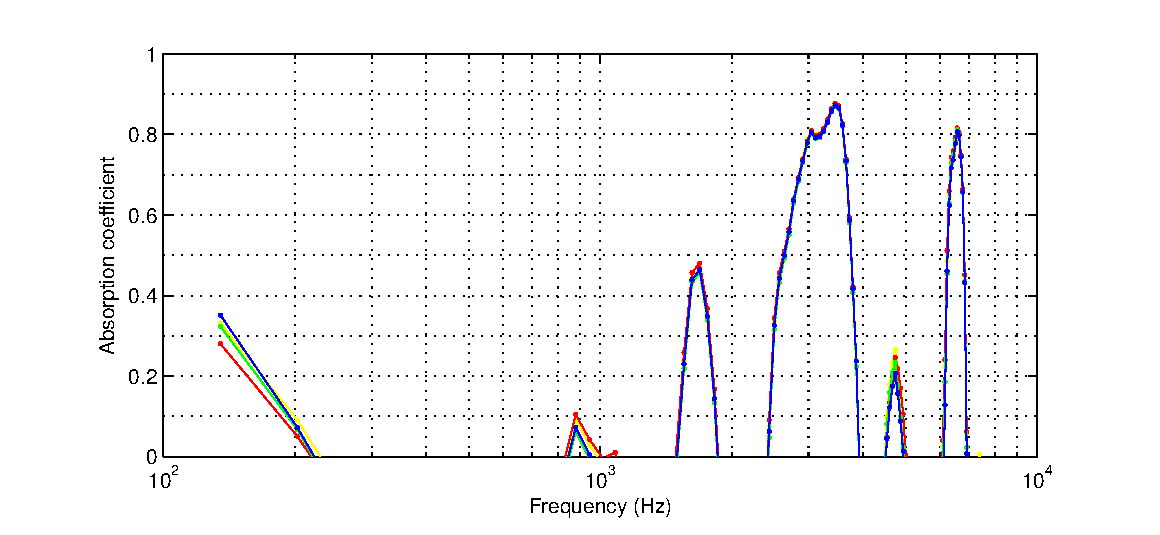
\includegraphics[width=\textwidth]{helmalles}
  %\vspace{-10pt}
  \caption{Absorption coefficient of the Helmholtz resonator determined with different excitation signals: 16$\times$ MLS of order 18 (yellow), 64$\times$ MLS of order 16 (red), 1$\times$ sweep of 60\,s (green), 64$\times$ sweep of 1\,s (blue).}
  \label{fig: helmholtzalles}
  %\vspace{-30pt}
\end{figure}


\subsection{The Adrienne method}
The acoustical characterisation of objects is an essential part in the design of noise reducing devices, such as the noise barriers along a motorway. It is important to be able to evaluate the performance of such barriers and more importantly to be able to compare them objectively. In order to do so a series of standardized methods was developed by CEN (European committee for standardization) to determine the performance of such devices. One of these methods determines the sound reflection of the device and is called the Adrienne method. A short description of the Adrienne method and its shortcomings will be given in this section. For more details, see the technical specification CEN/TS 1793-5:2003 \cite{Adrienne}.



\subsubsection{Experimental setup}

\begin{wrapfigure}{r}[0.08\textwidth]{0.4\textwidth}
	\vspace{-40pt}
  \centering
    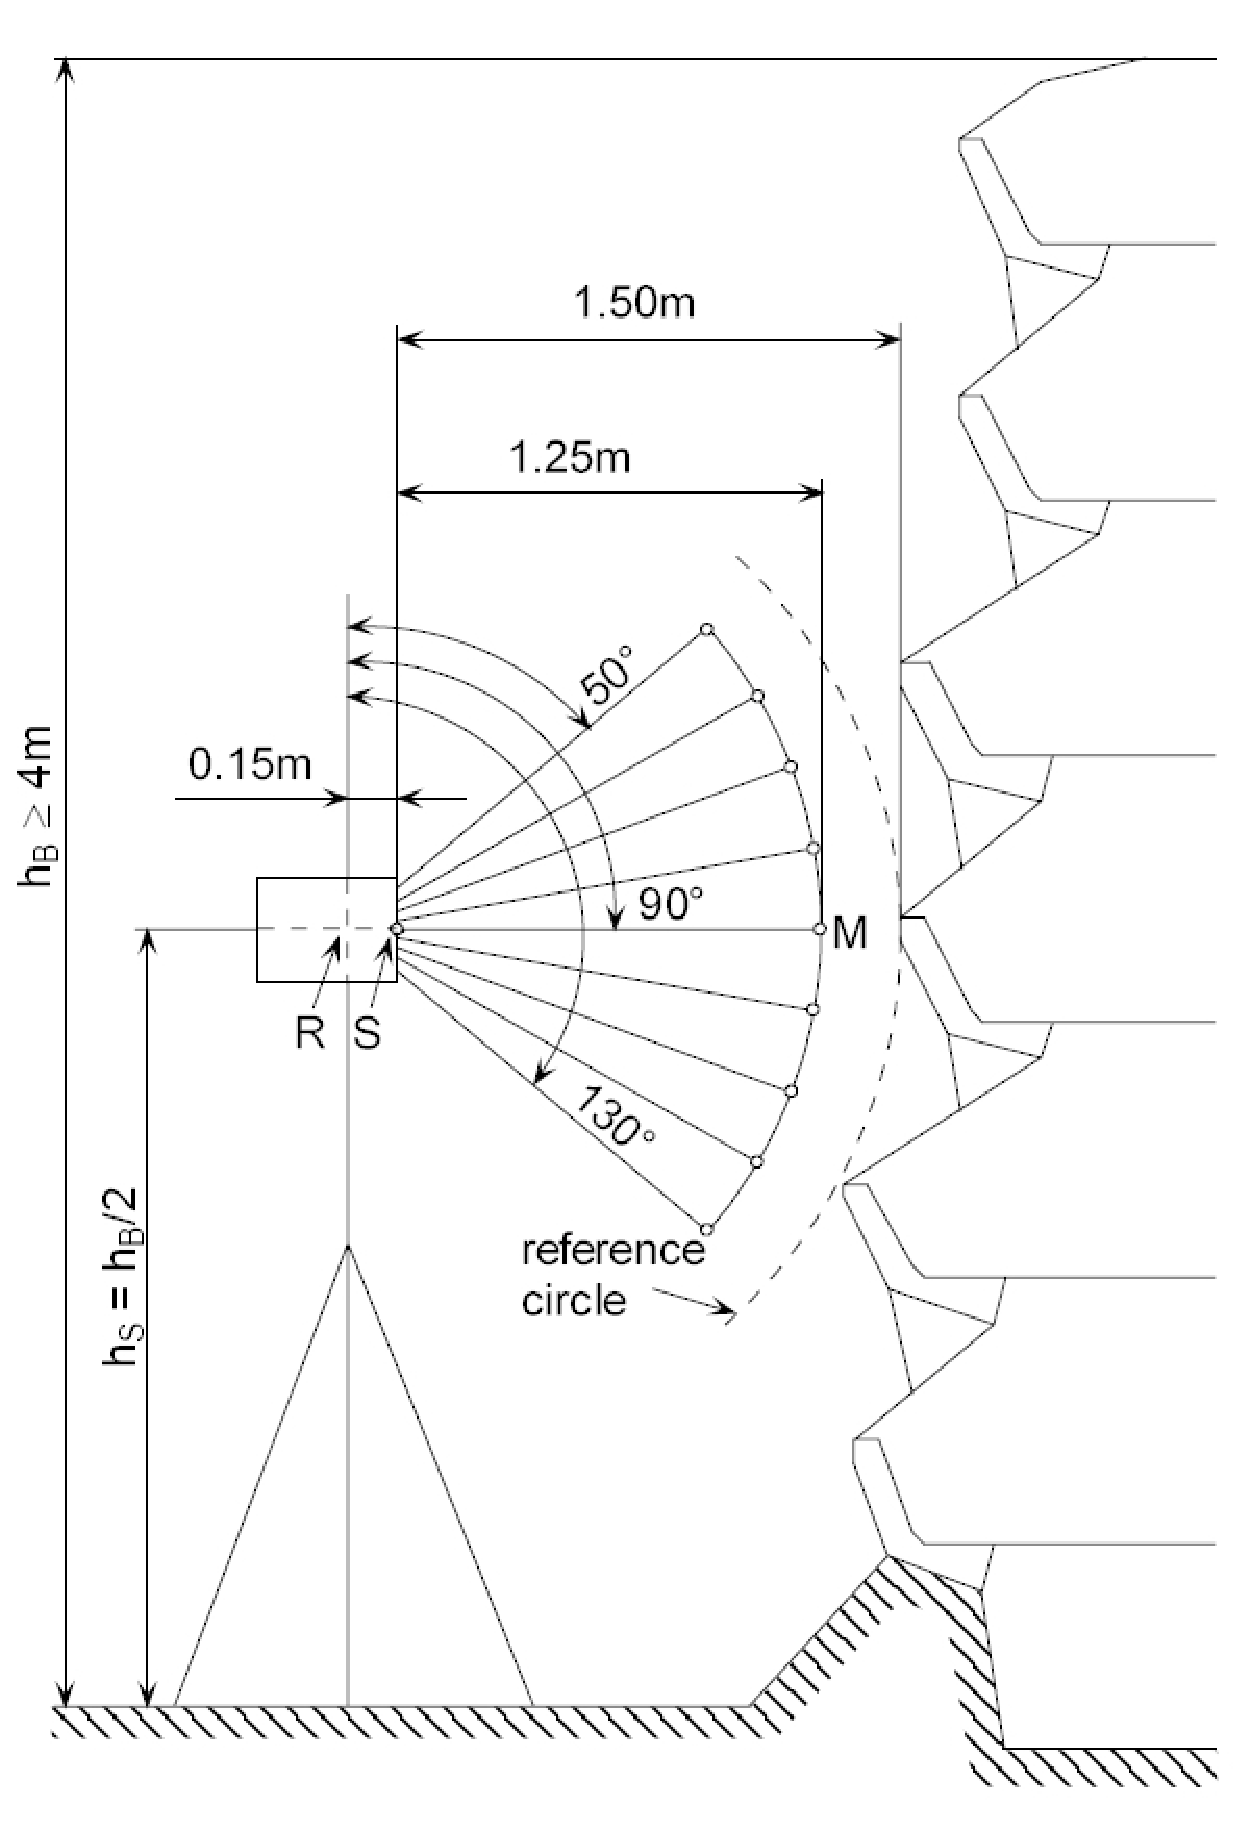
\includegraphics[width=0.4\textwidth]{Adrienne.pdf}
  \caption{Setup for the reflection index measurements according to the Adrienne method.}
  \label{fig: adrienne}
  \vspace{-40pt}
\end{wrapfigure}
The Adrienne method requires the setup shown in figure \ref{fig: adrienne}\footnote{This image was taken from \cite[p.45]{Geetere}.}. The microphone is attached to the speaker, such that the distance between them is 1.25m. The speaker is placed at a distance of 1.50\,m of the wall. The speaker and microphone assembly are capable of rotating. A set of nine measurement is performed with the angle varying between $50\degr$ and $130\degr$ in steps of $10\degr$.  Several sets of measurement have to be executed at different positions and rotating along different axes dependent on the homogeneity of the sample.
The excitation signal is a MLS and the signal is averaged at least 16 times.


\subsubsection{Data processing}\label{adrwindow}
The processing of the data happens as follows: the impulse response of a measurement is determined using cross correlation. The reflected component is extracted from the total impulse response by subtracting the direct component (obtained from a free field measurement). A time window is placed on the reflected component to remove parasitic reflections (for example from the floor). The window selected for this purpose is called the Adrienne temporal window and it has the following specifications \cite{Adrienne}:
%\vspace{-20pt}
\begin{itemize}
	\setlength{\itemsep}{1pt}
  \setlength{\parskip}{0pt}
  \setlength{\parsep}{0pt}
	\item a leading edge of 0.5\,ms with a left-half Blackman-Harris shape,
	\item a flat portion of length 5.18\,ms,
	\item a trailing edge of 2.22\,ms with a right-half Blackman-Harris shape.
\end{itemize}
%\vspace{-20pt}
The full Blackman-Harris window of length T is defined as 
\[
w(t) = 0.35875 - 0.48829 \cos(\frac{2 \pi t}{T}) + 0.14128 \cos(\frac{4 \pi t}{T}) - 0.01168 \cos(\frac{6 \pi t}{T}).
\]
This window shall be placed such that its flat portion begins 0.2\,ms before the first peak of the needed impulse response.

With these ingredients a parameter called the reflection index of the device under test is computed in 1/3 octave bands using the following formula 
\begin{equation}
RI_j = \frac{1}{n_j} \sum^{n_j}_{k=1} \frac{\int_{\Delta f_j} \left|\mathcal{F}\left[t\cdot h_{r,k}(t)\cdot w_r(t)\right]\right|^2 \,df }{\int_{\Delta f_j} \left|\mathcal{F}\left[t \cdot h_{i}(t) \cdot w_i(t)\right]\right|^2 \,df }
\label{RI}
\end{equation}
with \\

\begin{tabular}{ll}
$h_i(t)$ & the free field impulse response \\
$h_{r,k}(t) = h_k(t) - h_i(t)$ & the reflected component of the impulse response at the k-th angle \\
$w_i(t)$ & the Adrienne window for the free field impulse response\\ 
$w_r(t)$ & the Adrienne window for the reflected component of the impulse response\\ 
$\mathcal{F}$ & the symbol for Fourier transform \\
$\Delta f_j$ & the width of the j-th one third octave frequency band\\
$n_j$ & the number of angles on which to average\\ 
\end{tabular}

The parameter $t$ which is added to both the numerator and denominator is necessary to correct for geometrical $1/r$ attenuation since $r =c t$. 
The reflection index is a measure for the average ratio of reflected energy and incident energy. It is this standardized quantity that is used to compare the reflection capacities of different noise barriers. For more details, see \cite{Adrienne}.

\subsubsection{Shortcomings}
\begin{wrapfigure}{r}{0.20\textwidth}
	\vspace{-10pt}
  \centering
    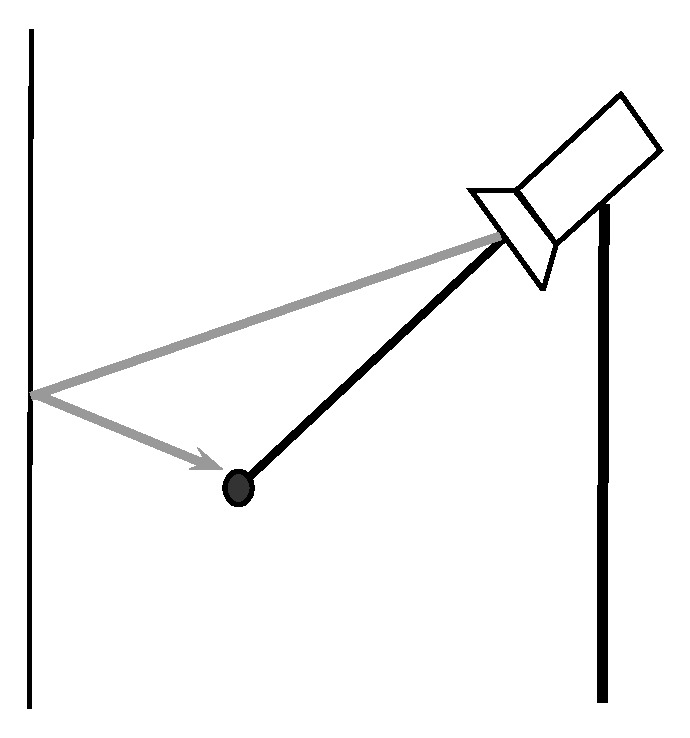
\includegraphics[width=0.20\textwidth]{adriennedir}
  \caption{Path of the reflected wave.}
  \label{fig: adriennedir}
  %\vspace{-40pt}
\end{wrapfigure}
The problem with the Adrienne method is that the directionality of the speaker is not accounted for. For example: when measuring at an angle of $130\degr$, the path of the reflected wave will resemble figure \ref{fig: adriennedir}. It is clear that the reflected component was emitted at a different angle than the direct component. Hence the reflected component contains a different speaker response. And this was only the case for a flat surface, imagine what would happen for non flat walls. Another disadvantage of this setup is that the speaker itself can be the cause of the first parasitic reflection which limits the time window, since it stands relatively close to the wall. Therefore, it would be advisedly to place the speaker at a greater distance from the wall and keep the microphone close to it.

This would not only solve the problem of parasitic reflections from the speaker, it would also reduce the influence of the speaker's directivity. The solid angle in which the response of the speaker can be considered as more or less equal remains the same, but the effective surface on the wall becomes larger. The angle between the direct sound path and the reflected sound path becomes smaller as the speaker is further removed of the wall. And hence the influence of the speaker's directivity diminishes.

\begin{wrapfigure}{r}{0.3\textwidth}
	%\vspace{-10pt}
  \centering
    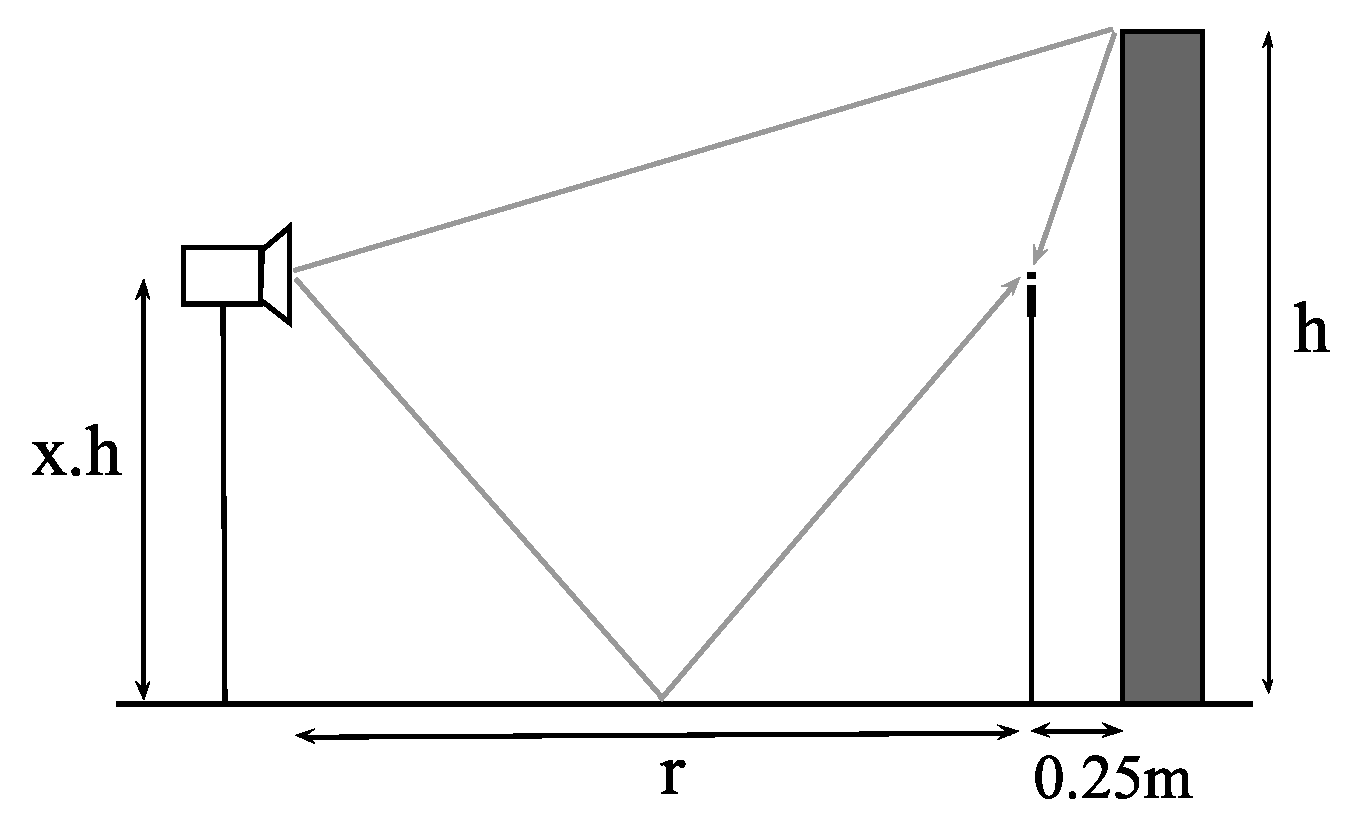
\includegraphics[width=0.3\textwidth]{hoger}
  \caption{Paths of the ground reflection and top diffraction.}
  \label{fig: hoger}
  %\vspace{-40pt}
\end{wrapfigure}
The disadvantage of placing the speaker further away, is that the ground reflection comes quicker after the reflected sound. This results in a shorter Adrienne window and consequently a larger lowest frequency limit. The solution to this problem would be to place the speaker and microphone higher. This, however, would cause the sound wave due to diffraction on the top of the wall to arrive sooner. But when considering the fact that the diffracted wave has to travel further than the ground reflection in the Adrienne case, the height of the microphone and speaker can be adjusted so that the ground reflection and the diffracted wave arrive at the same time (see figure \ref{fig: hoger}). In the case of a wall of 4 meters high, the speaker is positioned at a height of 2\,m according to the Adrienne setup and the first parasitic reflection arrives 7.91\,ms after the reflection of the wall. When placing the speaker at 2\,m from the microphone instead of 1.25\,m, the optimal height is 2.16\,m and the first parasitic reflection arrives 7.38\,ms after the wall reflection. The lowest measurable frequency is 160\,Hz for the Adrienne method and 170\,Hz for the adapted version\footnote{The lowest measurable frequency is calculated as $\frac{1}{0.8 T}$ with T the length of the Adrienne window \cite[p.70]{Geetere}.}. Since both belong to the 200\,Hz 1/3 octave band, the loss in frequency range is minimal, but the gain in accuracy is substantial. As will be shown in section \ref{insitu}.




\subsection{In situ measurement}\label{insitu}
\begin{wrapfigure}{r}{0.25\textwidth}
	\vspace{-10pt}
  \centering
    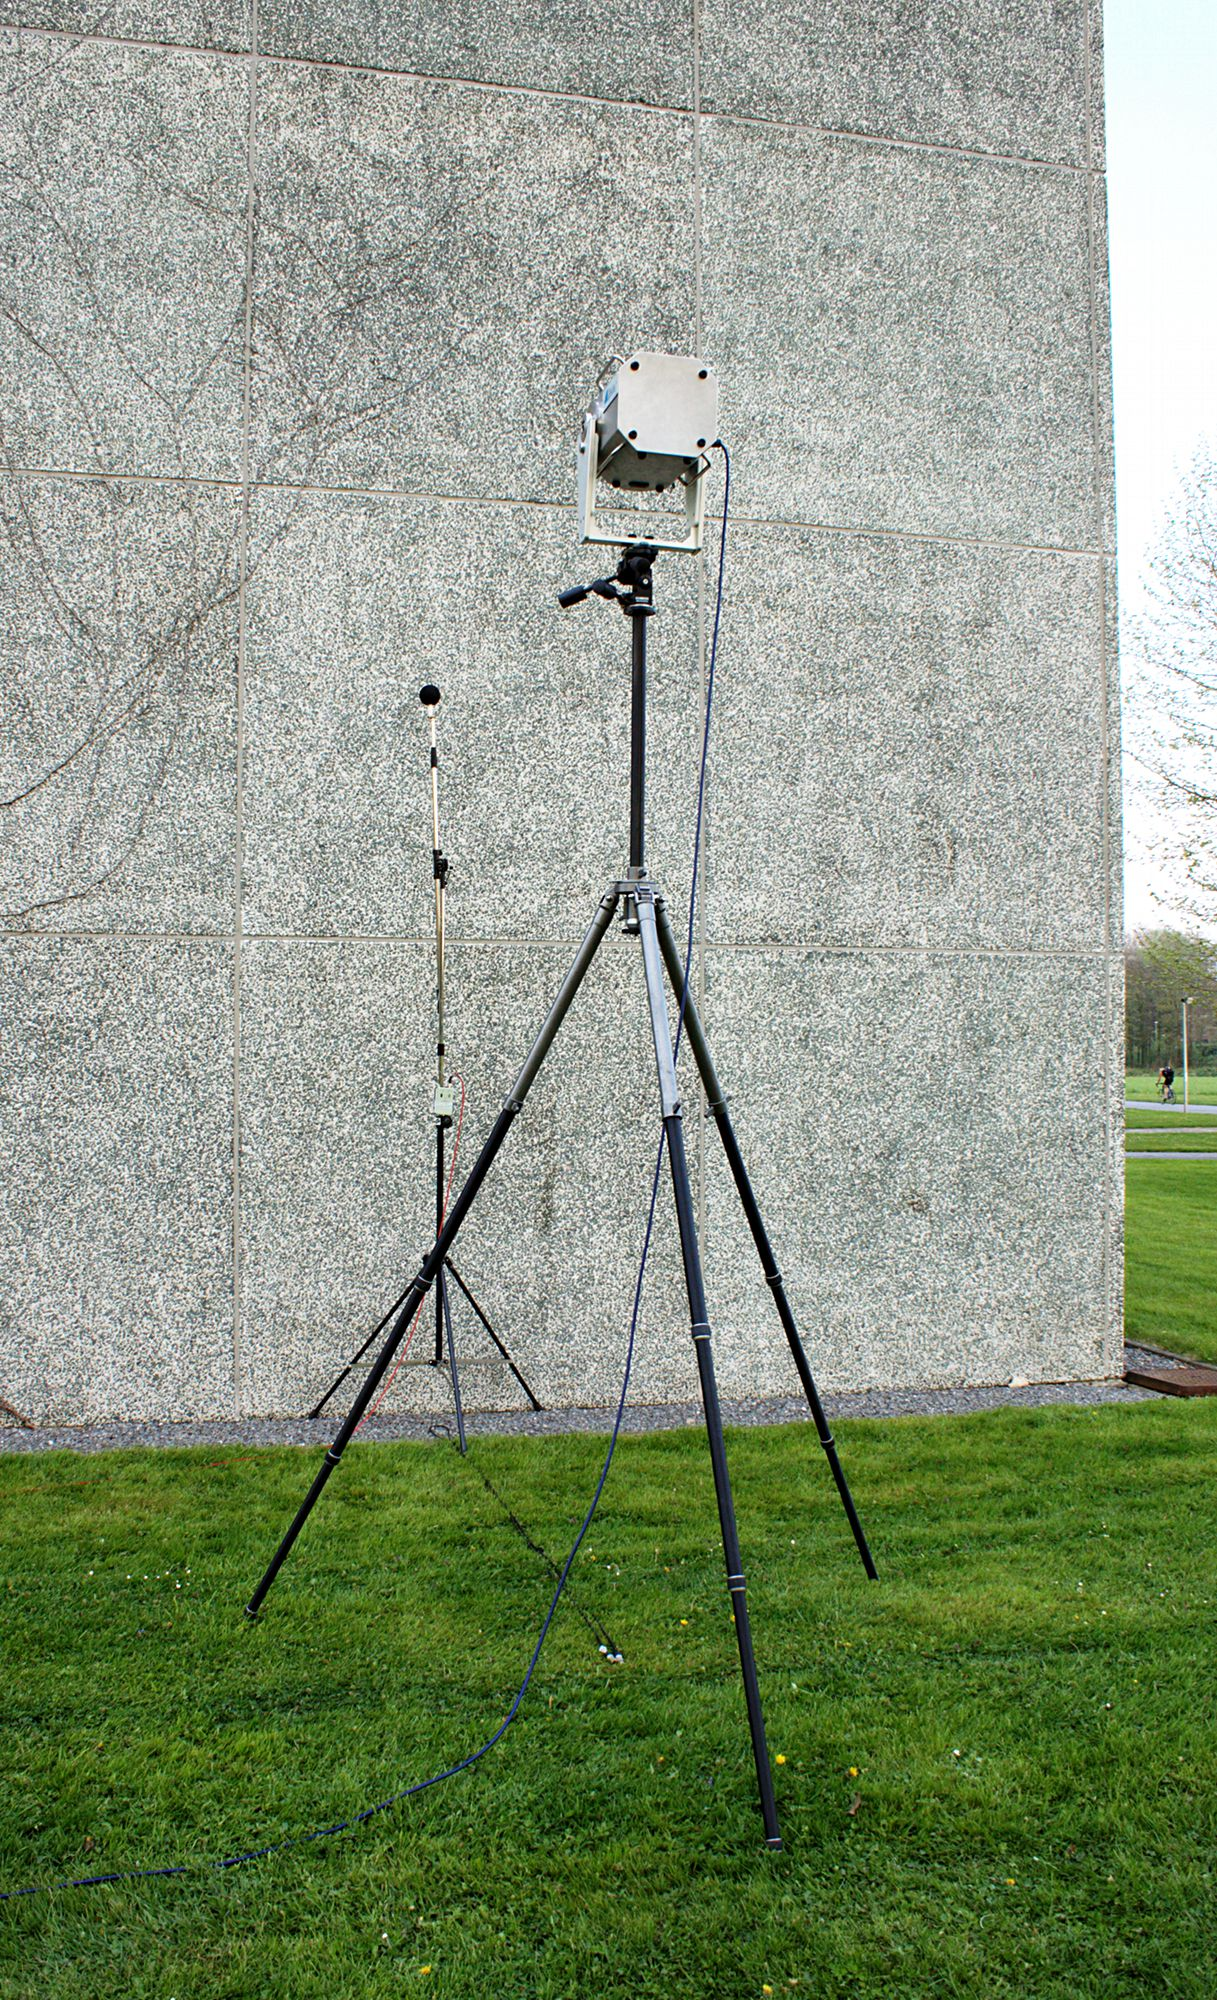
\includegraphics[width=0.25\textwidth]{wallOutside}
  \caption{Picture of the wall and setup.}
  \label{fig: wall}
  %\vspace{-40pt}
\end{wrapfigure}
Originally, a measurement of the reflection coefficient of a noise barrier along a highway in Brussels was planned, but due to unforeseen circumstances this field trip was cancelled. As a replacement, we decided to put the Adrienne method to the test. As test subject we chose the external concrete wall of the acoustics lab at the KULeuven. The reflection index of this wall was determined with the Adrienne method by L. De Geetere \cite[p.68]{Geetere}. His results are plotted in figure ref{fig: geetere}. Our goal is to ascertain the reflection coefficient of the wall while considering the directivity of the Zircon speaker and compare it with the Adrienne results (this can be done because De Geetere used the same Zircon speaker). 

Our experimental setup consisted of the following: the speaker and microphone are positioned at a (maximum) height of 3.15\,m and at a mutual distance of 3\,m. The microphone is placed at 0.25\,m of the wall. The setup and wall are shown in figure \ref{fig: wall}. This arrangement makes sure that the first parasitic reflection arrives 10\,ms after the wall reflection. Since the measurements are done in a noisy environment, the excitation signal is an MLS of order 16 and is averaged 64 times. To make sure that no distortion peaks occurred in the relevant time domain, a measurement was done with a sine sweep signal and subtracted. This revealed that the distortion peaks did not contaminate the important part of the impulse response. 

\begin{wrapfigure}{r}{0.40\textwidth}
	\vspace{-10pt}
  \centering
    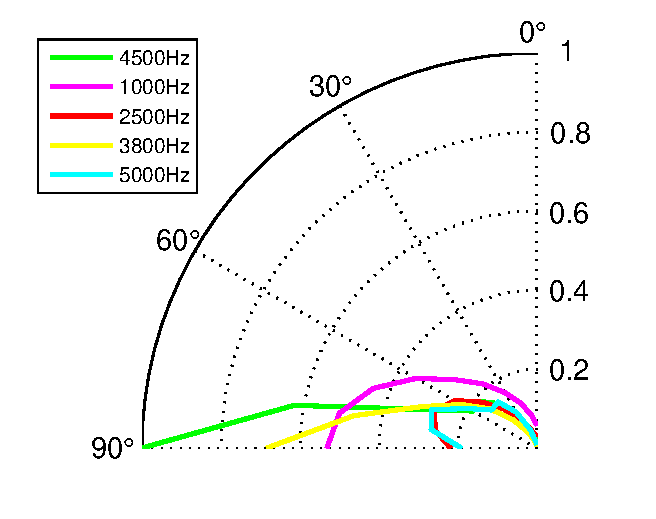
\includegraphics[width=0.40\textwidth]{polar}
  \caption{Angular dependence of the frequency response of the speaker for certain frequencies.}
  \label{fig: polar}
  %\vspace{-40pt}
\end{wrapfigure}
A set of measurements was performed at horizontal angles of $90\degr$, $100\degr$, $110\degr$ and $120\degr$. This was done by keeping the microphone at the same place and moving the speaker. The results of this set are shown in figure \ref{fig: wallref}. Below 400\,Hz the reflection coefficient can not be considered accurate, as these spectral bands are only populated by a single data point. It is clear that there are some dissimilarities between the graphs: the Adrienne result contains dips at 1000\,Hz and 4000\,Hz, whereas our results remain approximately one. This discrepancy can be explained by looking at figure \ref{fig: thetavar} and formula \ref{RI}: the reflection index is calculated using the free field measurement as normalization for the 1/3 octave bands. For angles other than $90\degr$, the wall receives a  speaker response which differs from the free field measurement as shown in figure \ref{fig: adriennedir}. And hence the normalization is not correct. Figure \ref{fig: polar} shows the angular dependence of the frequency response of the speaker for several frequencies. The values at $90\degr$ correspond to the free field spectrum. For 4500Hz, 3800Hz and 1000Hz, the frequency response decreases as $\theta$ deviates from $90\degr$. Hence the calculated reflection index is an underestimate, which explains the dips in figure \ref{fig: geetere}. For 2500Hz and 5000Hz, the frequency response increases as $\theta$ deviates from $90\degr$, thus the calculated reflection index is an overestimate, which explains the increase of the reflection index at 2500Hz and 5000Hz. 

\begin{figure}[h!]
  \centering
  \subfigure[Our method]{\label{fig: wallref}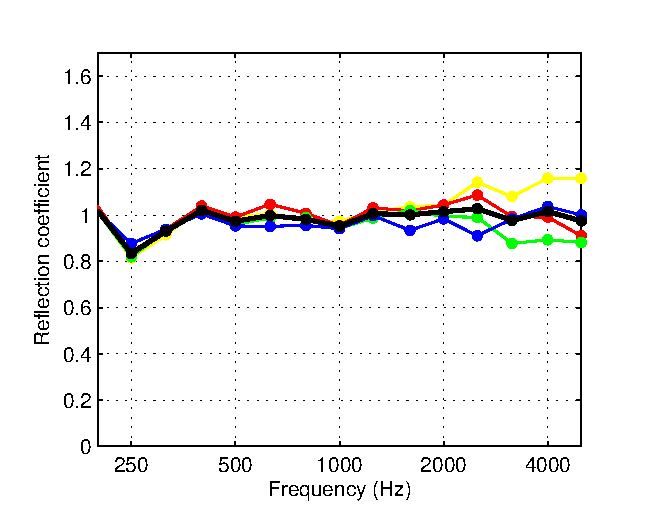
\includegraphics[width=0.45\textwidth]{wallref}}                
  \subfigure[Adrienne method]{\label{fig: geetere}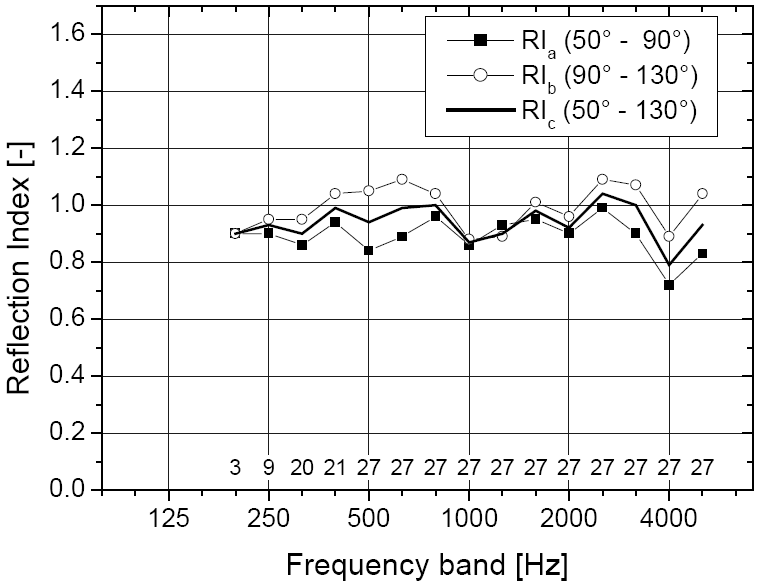
\includegraphics[width=0.45\textwidth]{geetere}}
  \caption{The reflection coefficient in 1/3 octave bands of the wall of the acoustics department at the KUL. On the left are the results of our measurements at $90\degr$ (yellow), $100\degr$ (red), $110\degr$ (green) and $120\degr$ (blue). The black line is the average of these 4 measurements. On the right are the results determined by L. de Geetere with the Adrienne method. The figure is taken from \cite[p.68]{Geetere}.}
  \label{fig: reflection}
\end{figure}



%\end{document}

\section{Conclusion}
In this paper, three methods to characterize the acoustical properties of a noise barrier were discussed. 

First, measurements on a scale model were explored. Care was taken to correct for spurious attenuation of high frequency components due to absorption from the air. Ways of dealing with the low signal to noise ratio were briefly touched.

These measurements were then compared to a simulation of the exact same setup using a basic time domain finite difference scheme. Noteworthy was the correction to 3D of the 2D simulation and the use of a staggered grid to improve accuracy without sacrificing performance.

The measured results appeared to match with the simulation rather well, at least on a coarse level. A closer look showed some slight deviations, possibly related to atmospheric attenuation or the difference between 2D and 3D for diffuse reflections. Nonetheless, the qualitative properties were very similar in both cases. Diffraction clearly manifested itself, as could be seen in the time domain and in the frequency domain as the characteristic 6\,dB per octave attenuation.

The third and final approach consists of measuring the acoustical performance of a life sized noise barrier. In order to do this, a program was written in Matlab to send and record sounds and to process the gathered data. The standard method for reflection measurements was assessed and it turned out that the Adrienne method does not account for the directivity of the loudspeaker.

In order to overcome this difficulty an alternative method was suggested, which involves placing the speaker higher and further away from the wall. Doing so results in a smaller frequency range, but the effect of the speaker's directivity is diminished. This improved method was used to determine the reflection coefficient of a concrete wall. The results were compared with those of the Adrienne method and it was found that the Adrienne method is subject to the directivity of the speaker, whereas the improved method gave a reflection coefficient of approximately one (as expected for a concrete wall). Although the improved method might not always be practical, it certainly is more physically correct.


% vim: spell spelllang=en_us



\clearpage
\footnotesize
\bibliographystyle{plain}
\bibliography{references}
\nocite{*}

\end{document}
